\chapter{Algebraic Curves}
\section{Algebraic Preliminaries}
\begin{proposition}
An algebraically closed field $k$ is infinite.
\end{proposition}
\begin{proof}
The irreducible polynomials of $k[x]$ are exactly $x-a,a\in k$. Assume that $k$ is finite, then consider the polynomial
\[F(x)=\prod_{a\in k}(x-a)+1.\]
Since $k$ is algebraically closed, $F(x)$ must have a root. But each element of $k$ is not a root of $F$.
\end{proof}
For a polynomial $F\in k[X_1,\dots,X_n]$, let $V(F)$ be the zero set of $F$.
\begin{proposition}
Let $k$ be an infinite field, $F\in k[X_1,\cdots,X_n]$. Then $F=0$ iff $F(a_1,\dots,a_n)=0$ for all $a_1,\dots,a_n\in k$.
\end{proposition}
\begin{proof}
Write $F=\sum F_iX_n^i$ with $F_i\in k[X_1,\dots,X_{n-1}]$. Then for any $a_1,\dots,a_{n-1}\in k$, by our hypothesis the polynomial $F(a_1,\dots,a_{n-1},X_n)$ vanish on $k$, hence is zero. This means each $F_i$ vanishes on all elements, and is therefore zero. Now use induction.
\end{proof}
\begin{proposition}\label{infinity V(F)}
Let $F$ be a nonconstant polynomial in $k[X_1,\dots,X_n]$, $k$ algebraically closed. Then $\mathbb{A}^n(k)-V(F)$ is infinite if $n\geq1$, and $V(F)$ is infinite if $n\geq2$.
\end{proposition}
\begin{proof}
Write $F=\sum F_iX_n^i$ with $F_i\in k[X_1,\dots,X_{n-1}]$. Since $k$ is algebraically closed, it is infinite.\par
Since $F\neq 0$, there exists a pair of elements $a_1,\dots,a_{n-1}\in k$ such that $F(a_1,\dots,a_{n-1},X_n)\neq 0$. Then since $V(F(a_1,\dots,a_{n-1},X_n))$ is finite, there are infinitely many elements $a\in k$ such that $F(a_1,\dots,a_{n-1},a)\neq 0$. This implies $\mathbb{A}^n(k)-V(F)$ is infinite.\par
Now assume $n\geq 2$, then for any pair of elements $a_1,\dots,a_{n-1}\in k$, the polynomial $F(a_1,\dots,a_{n-1},X_n)$ has a root $a_n$. Since then $(a_1,\dots,a_n)\in V(F)$, we conclude $V(F)$ is infinite. 
\end{proof}
\subsection{Forms}
Let $R$ be a domain. If $F\in R[X_1,\dots,X_{n+1}]$ is a form, we define $F_*\in R[X_1,\dots,X_{n}]$ by setting $F_*=F(X_1,\dots,X_n,1)$. Conversely, for any polynomial $f\in R[X_1,\dots,X_n]$ of degree $d$, write $f=f_0+\cdots+f_d$, where $f_i$ is a form of degree $i$, and define $f^*\in R[X_1,\dots,X_{n+1}]$ by setting
\[f^*=\sum_{i=0}^{d}X_{n+1}^{d-i}f_{i}=X_{n+1}^df(X_1/X_{n+1},\dots,X_n/X_{n+1}).\]
$f^*$ is a form of degree $d$. (These processes are often described as \textbf{dehomogenizing} and \textbf{homogenizing} polynomials with respect to $X_{n+1}$.) The following proposition holds.
\begin{proposition}\label{homogenousing}
With notations above.
\begin{itemize}
\item $(FG)_*=F_*G_*$, $(F+G)_*=F_*+G_*$.
\item $(fg)^*=f^*g^*$, while $X_{n+1}^t(f+g)^*=X_{n+1}^rf^*+X_{n+1}^sg^*$, where $r=\deg g,s=\deg f$ and $t=r+s-\deg(f+g)$.
\item If $F\neq 0$ and $\ell$ is the highest power of $X_{n+1}$ that divides $F$, then $X_{n+1}^\ell(F_*)^*=F$; $(f^*)_*=f$.
\end{itemize}
\end{proposition}
\begin{proof}
From the definition of $F_*$, it is clear that $(FG)_*=F_*G_*,(F+G)_*=F_*+G_*$. Now let $\deg f=s$ and $\deg g=r$, we have
\[(fg)^*=X_{n+1}^{r+s}(fg)(X_1/X_{n+1},\dots,X_n/X_{n+1})=f^*g^*.\]
and
\begin{align*}
X_{n+1}^t(f+g)^*&=X_{n+1}^{\deg(f+g)+t}(f+g)(X_1/X_{n+1},\dots,X_{n}/X_{n+1})\\
&=X_{n+1}^{r+s}f(X_1/X_{n+1},\dots,X_{n}/X_{n+1})+X_{n+1}^{r+s}g(X_1/X_{n+1},\dots,X_{n}/X_{n+1})\\
&=X_{n+1}^rf^*+X_{n+1}^sg^*.
\end{align*}
Finally, it is clear that $(f^*)_*=f$, for the second part, note that
\[\deg F_*=\deg F-\ell,\]
therefore
\begin{align*}
X_{n+1}^\ell(F_*)^*&=X_{n+1}^\ell X_{n+1}^{\deg F_*}F(X_1/X_{n+1},\dots,X_n/X_{n+1},1)\\
&=X_{n+1}^{\deg F}F(X_1/X_{n+1},\dots,X_n/X_{n+1},1)=F.\end{align*}
where we use thefact that $F$ is a form.
\end{proof}
\begin{corollary}\label{factor k[X,Y]}
Up to powers of $X_{n+1}$, factoring a form $F\in R[X_1,\dots,X_{n+1}]$ is the same as factoring $F_*\in R[X_1,\dots,X_n]$. In particular, if $F\in k[X,Y]$ is a form, $k$ algebraically closed, then $F$ factors into a product of linear factors.
\end{corollary}
\begin{proof}
The first claim follows directly from the previous proposition. For the
second, write $F=Y^rG$, where $Y$ doesn't divide $G$. Then $F_*=G_*=c\prod(X-\lambda_i)$ since $k$ is algebraically closed, so $F=cY^r\prod(X-\lambda_i Y)$.
\end{proof}
\section{Affine Algebraic Sets}
\subsection{Affine Space and Algebraic Sets}
Let $k$ be any field. By $\mathbb{A}^n(k)$, or simply $\mathbb{A}^n$ (if $k$ is understood), we shall mean the cartesian product of $k$ with itself $n$ times: $\mathbb{A}^n(k)$ is the set of $n$-tuples of elements of $k$. We call $\mathbb{A}^n(k)$ \textbf{affine $\bm{n}$-space over $\bm{k}$}; its elements will be called points. In particular, $\mathbb{A}^1(k)$ is the affine line, $\mathbb{A}^2(k)$ the affine plane.\par 
If $F\in k[X_1,\dots,X_n]$, a point $P=(a_1,\dots,a_n)$ in $\mathbb{A}^n(k)$ is called a zero of $F$ if $F(P)=F(a_1,\dots,a_n)=0$. If $F$ is not a constant, the set of zeros of $F$ is called the \textbf{hypersurface defined by $\bm{F}$}, and is denoted by $V(F)$. A hypersurface in $\mathbb{A}^2(k)$ is called an \textbf{affine plane curve}. If $F$ is a polynomial of degree one, $V(F)$ is called a \textbf{hyperplane} in $\mathbb{A}^n(k)$.
\begin{example}
Let $k=\R$.
\[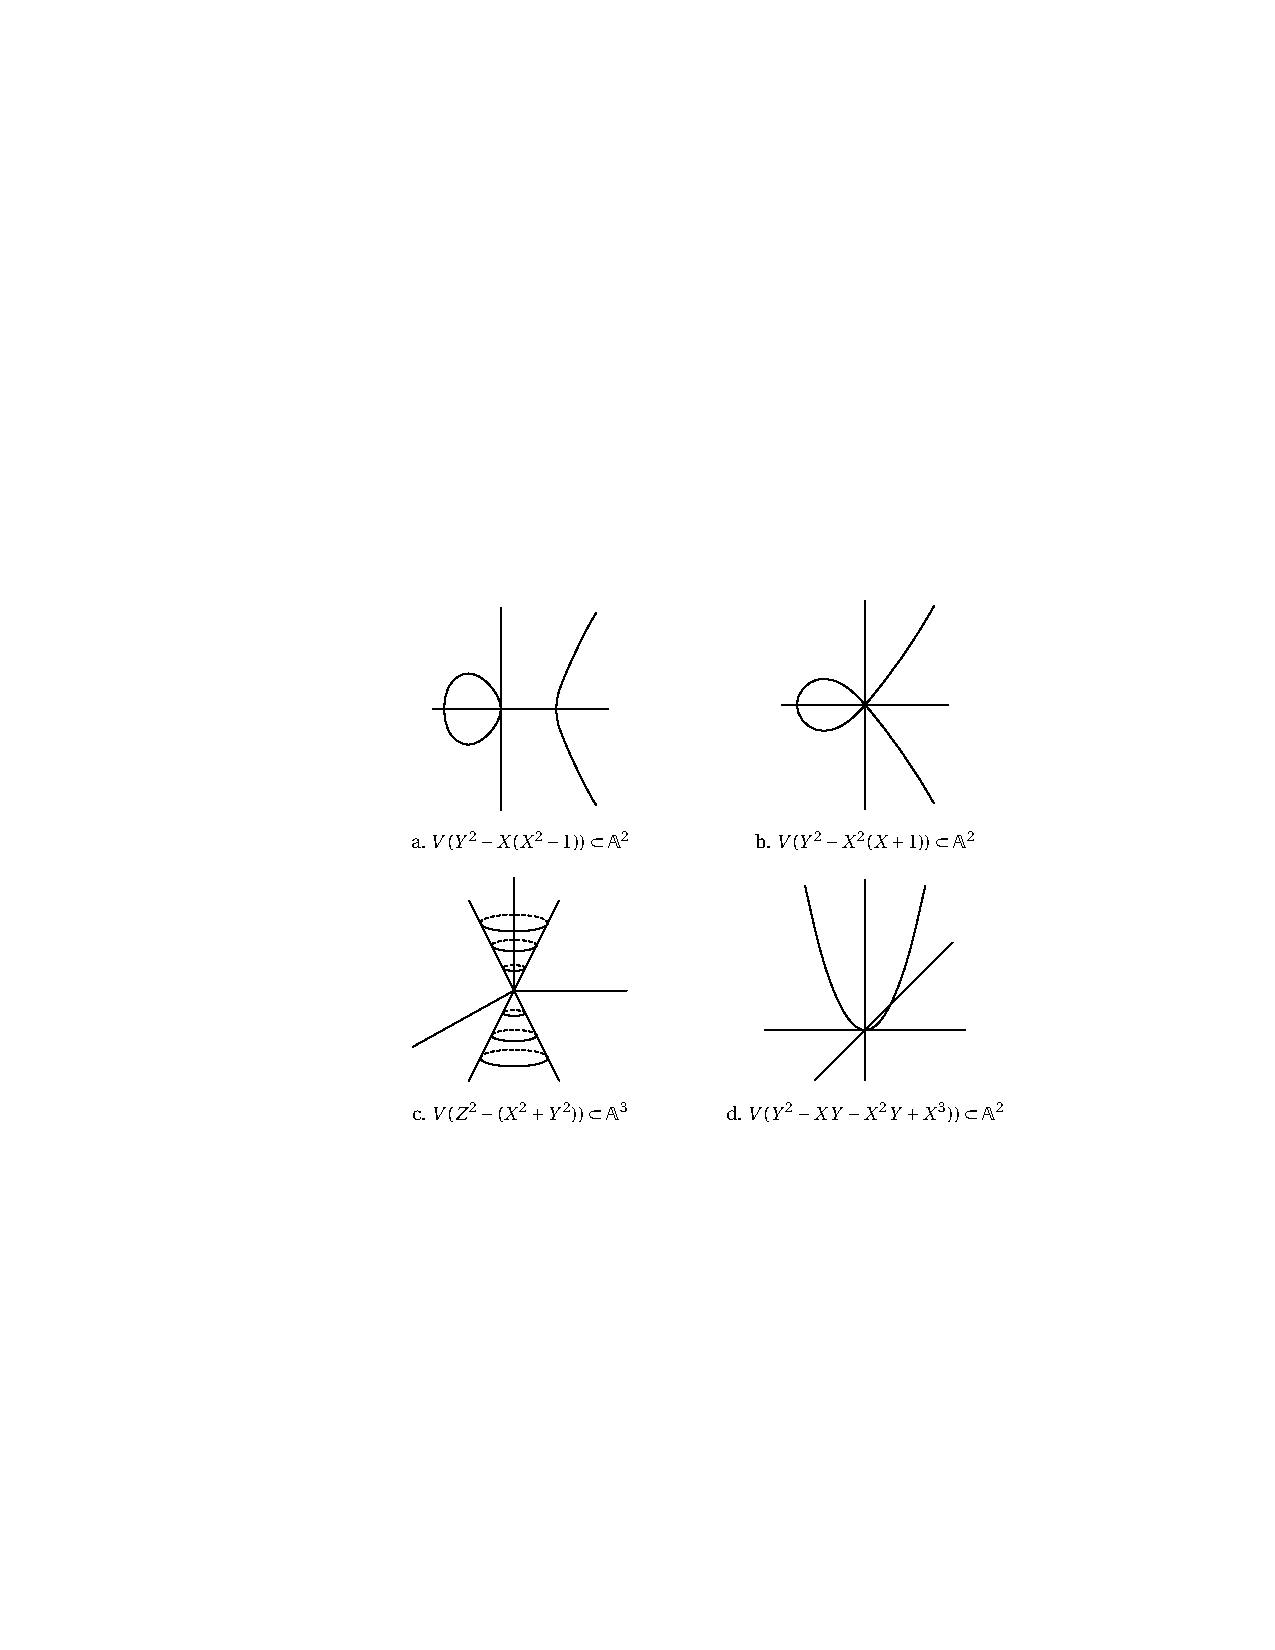
\includegraphics{pictures/algebraic-set}\]
\end{example}
More generally, if $S$ is any set of polynomials in $k[X_1,\dots,X_n]$, we let 
\[V(S)=\{P\in\mathbb{A}^n:F(P)=0\text{ for all }F\in S\}=\bigcap_{F\in S}V(F).\]
If $S=\{F_1,\dots,F_r\}$, we usually write $V(F_1,\dots,F_r)$ instead of $V(\{F_1,\dots,F_r\})$. A subset $X\sub\mathbb{A}^n(k)$ is an \textbf{affine algebraic set}, or simply an \textbf{algebraic set}, if $X=V(S)$ for some $S$.
\begin{proposition}
Let $k$ be a field.
\begin{itemize}
\item[$(1)$] If $I\sub J$, then $V(J)\sub V(I)$.
\item[$(2)$] If $I$ is the ideal in $k[X_1,\dots,X_n]$ generated by $S$, then $V(S)=V(I)$; so every algebraic set is equal to $V(I)$ for some ideal $I$.
\item[$(3)$] If $\{I_\alpha\}_{\alpha\in A}$ is any collection of ideals, then $V(\bigcup_\alpha I_\alpha)=\bigcap_\alpha V(I_\alpha)$; so the intersection of any collection of algebraic sets is an algebraic set. 
\item[$(4)$] $V(FG)=V(F)\cup V(G)$ for any polynomials $F,G$; $V(I)\cup V(J)=V(IJ)$ for ideals $I,J$; so any finite union of algebraic sets is an algebraic set.
\item[$(5)$] $V(0)=\mathbb{A}^n(k)$; $V(1)=\emp$. $V(X_1-a_1,\dots,X_n-a_n)=\{(a_1,\dots,a_n)\}$ for $a_i\in k$. So any finite subset of $\mathbb{A}^n(k)$ is an algebraic set.
\end{itemize}
\end{proposition}
\begin{proof}
The first statement follows from the definition. For the second, it is clear that $V(I)\sub V(S)$. Assume $P\in V(S)$, then since any element of $I$ is a linear combination of $S$, we also have $P\in V(I)$. Thus $V(I)=V(S)$.\par
Now for a family $\{I_\alpha\}$, we have
\[V(\bigcup_\alpha I_\alpha)=\bigcap_{F\in\bigcup I_\alpha}V(F)=\bigcap_{\alpha}\bigcap_{F\in I_\alpha}V(F)=\bigcap_{\alpha}V(I_\alpha),\]
as needed.\par
If $F(P)G(P)=0$, then $F(P)=$ or $G(P)=0$, thus the equality $V(FG)=V(F)\cup V(G)$ holds. Now for ideals $I,J$, we observe
\[V(F)\cup V(G)=\bigcap_{F\in I}V(F)\cup\bigcap_{G\in J}V(G)=\bigcap_{F\in I,G\in J}(V(F)\cup V(G))=\bigcap_{F\in I,G\in J}V(FG)=V(IJ).\]
The last staement is immediate.
\end{proof}
Generally, a infinite union of algebraic sets may not be algebraic. Here is an example.
\begin{example}
Let $k=\R$ and consider the subset $\Q\sub\R$. We observe that $\Q$ is not algebraic: if $\Q=V(S)$, then any polynomial in $S$ vanishes on $\Q$, hence on $\R$ by continuity. This means $S$ can only be zero, but $V(0)=\R$, contradiction. Since $\Q$ is itself contable, it is a countable union of algebraic sets.
\end{example}
\subsection{The Ideal of a Set of Points}
For any subset $X$ of $\mathbb{A}^n(k)$, we consider those polynomials that vanish on $X$; they form an ideal in $k[X_1,\dots,X_n]$, called the ideal of $X$, and written $I(X)$:
\[I(X)=\{F\in k[X_1,\dots,X_n]:F(a_1,\dots,a_n)=0\text{ for all }(a_1,\dots,a_n)\in X\}\]
\begin{proposition}
Let $k$ be a field.
\begin{itemize}
\item[$(1)$] If $X\sub Y$, then $I(Y)\sub I(X)$.
\item[$(2)$] $I(\emp)=k[X_1,\dots,X_n]$; $I(\mathbb{A}^n(k))=(0)$ if $k$ is infinite. 
\item[$(3)$] $I(\bigcup_\alpha S_\alpha)=\bigcap_\alpha I(S_\alpha)$.
\item[$(4)$] $I(\{(a_1,\dots,a_n)\})=(X_1-a_1,\dots,X_n-a_n)$ for $a_1,\dots,a_n\in k$.
\item[$(5)$] $I(X)$ is a radical ideal.
\item[$(6)$] For any ideal $I$ in $k[X_1,\dots,X_n]$, $V(I)=V(\sqrt{I})$, and $\sqrt{I}\sub I(V(I))$.
\item[$(7)$] $I(V(S))\sups S$ for any set $S$ of polynomials; $V(I(X))\sups X$ for any set $X$ of points.
\item[$(8)$] $V(I(V(S)))=V(S)$ for any set $S$ of polynomials, and $I(V(I(X)))=I(X)$ for any set $X$ of points. So if $V$ is an algebraic set, $V=V(I(V))$, and if $I$ is the ideal of an algebraic set, $I=I(V(I))$.
\end{itemize}
\end{proposition}
\begin{proof}
It is clear that if $F^n(P)=0$, then $F(P)=0$. Therefore $I(X)$ is a radical ideal and $V(I)=V(\sqrt{I})$. It is also clear that $I\sub I(V(I))$, so by taking radical we get $\sqrt{I}\sub I(V(I))$.\par
For $F\in k[X_1,\dots,X_n]$, $F\in I(\bigcup_\alpha S_\alpha)$ iff $F(P)=0$ for all $P\in\bigcup_\alpha S_\alpha$, iff $F\in I(S_\alpha)$ for all $\alpha$. Thus $I(\bigcup_\alpha S_\alpha)=\bigcap_\alpha I(S_\alpha)$.\par
For $S\sub k[X_1,\dots,X_n]$, from $(7)$ we get
\[I(V(S))\sups S\And V(I(V(S)))\sups V(S).\] 
Form the former we derive $V(I(V(S))\sub V(S)$, thus $V(I(V(S)))=V(S)$.
\end{proof}
\begin{corollary}
Let $V,W$ be algebraic sets in $\mathbb{A}^n(k)$. Then $V=W$ if and only if $I(V)=I(W)$.
\end{corollary}
\begin{proof}
For algebraic sets $V$ we have $V(I(V))=V$. Thus the map $I$ is injective.
\end{proof}
\begin{proposition}
Let $W$ be a subset of $\mathbb{A}^n$. Then $V(I(W))$ is the smallest algebraic subset of $\mathbb{A}^n$ containing $W$.
\end{proposition}
\begin{proof}
Certainly $V(I(W))$ is an algebraic set containing $W$. Let $V=V(J)$ be another algebraic set containing $W$. Then $J\sub I(V(J))\sub I(W)$, and so $V(J)\supset V(I(W))$.
\end{proof}
\begin{proposition}\label{algebraic set separate}
Let $V$ be an algebraic set in $\mathbb{A}^n(k)$.
\begin{itemize}
\item[$(a)$] If $P\in\mathbb{A}^n(k)$ is a point not in $V$, then there is a polynomial $F\in k[X_1,\dots,X_n]$ such that $F(Q)=0$ for all $Q\in V$, but $F(P)=1$.
\item[$(b)$] Let $P_1,\dots,P_r$ be distinct points of $\mathbb{A}^n(k)$ not in $V$. Then there are polynomials $F_1,\dots,F_r\in I(V)$ such that $F_i(P_j)=0$ if $i\neq j$, and $F_i(P_i)=1$.
\item[$(c)$] With $P_1,\dots,P_r$ as in $(b)$, and $a_{ij}\in k$ for $1\leq i,j\leq r$, there are $G_i\in I(V)$ with $G_i(P_j)=a_{ij}$ for all $i$ and $j$.
\end{itemize} 
\end{proposition}
\begin{proof}
Write $V=V(I)$. For any point $P\notin V$ there is a polynomial $F\in I$ such that $F(P)\neq 0$. Then $F'=F/F(P)$ satisfies the condition.\par
For $(b)$, apply $(a)$ to the union of $V$ and all but one point. And for $(c)$, consider the sum $G_i=\sum_j a_{ij}F_j$.
\end{proof}
\subsection{The Zariski topology}
\begin{definition}
We endow a topology on $\mathbb{A}^n(k)$ by declearing a subset is closed iff it is algebraic. This is called the \textbf{Zariski topology} on $\mathbb{A}^n$.
\end{definition}
A basis for the open subsets of $\mathbb{A}^n$ is given by the open sets
\[\mathbb{A}^n_f=D(f)=\mathbb{A}^n-V(f)=\{x\in\mathbb{A}^n:f(x)\neq 0\}.\]
with $f\in k[X_1,\dots,X_n]$. Open subsets of this type, complements of hypersurfaces in $\mathbb{A}^n$, are called \textbf{principal open} or \textbf{basic open subsets} of $\mathbb{A}^n$. Note that $D(f_1)\cap D(f_2)=D(f_1f_2)$.\par
Let us now examine some properties of the Zariski topology.
\begin{itemize}
\item $\mathbb{A}^n$ is not a Hausdorff space, because for every pair of non-empty open sets $U_1$, $U_2$ one has $U_1\cap U_2\neq\emp$. Indeed, if $U_1\cap U_2=\emp$, one would have $\mathbb{A}^n=U_1^c\cup U_2^c$. Since $\mathbb{A}^n$ is irreducible one would have either $U_1^c=\emp$ or $U_2^c=\emp$. It follows that every non-empty open set is dense in $\mathbb{A}^n$.
\item $\mathbb{A}^n$ is a Fr\'echet space (i.e., $T_1$) in the sense that if $P$ and $Q$ are any two distinct points, each of the two is contained in an open set which does not contain the other. In fact, if $f$ is a polynomial satisfying $f(P)\neq 0$ but $f(Q)=0$, then the open set which is the complement of the algebraic set $V(f)$ contains $P$ but not $Q$.
\item $\mathbb{A}^n$ is compact, that is, every open cover admits a finite subcover. From $\mathbb{A}^n=\bigcup_\alpha D(f_\alpha)$ we get
\[V(\bigcup_\alpha\{f_\alpha\})=\bigcap_\alpha V(f_\alpha)=\emp.\]
Since $k[X_1,\dots,X_n]$ is noetherian, there exists a finite set $f_1,\dots,f_n$ such that \[V(f_1,\dots,f_n)=V(\bigcup_\alpha\{f_\alpha\})=\emp.\] 
Thus we have $\mathbb{A}^n=\bigcup_{i=1}^{n}D(f_i)$.
\end{itemize}
If $V\sub\mathbb{A}^n$ is an algebraic set, we can consider the Zariski topology on $V$, namely the topology on $V$ induced by the Zariski topology on $\mathbb{A}^n$. For each $f\in k[V]$ we set
\[V_f=V-V(f)=\{P\in V:f(x)\neq 0\}.\]
The open sets $V_f$ are called \textbf{principal open} or \textbf{basic open subsets} of $V$, and form a base for the open subsets of the Zariski topology on $V$.
\begin{remark}
Let $V\in\mathbb{A}^n(k),W\in\mathbb{A}^m(k)$ be algebraic sets. Then
\[V\times W=\{(a_1,\dots,a_n,b_1,\dots,b_m):(a_1,\dots,a_n)\in V,(b_1,\dots,b_m)\in W\}\]
is an algebraic set in $\mathbb{A}^{n+m}(k)$. It is called the product of $V$ and $W$. In fact, rite $V=V_n(S)$ and $W=V_m(T)$. Note that we can embed $S$ and $T$ in $k[X_1,\dots,X_{n+m}]$, and one can verify the equality $V\times W=V(S^e)\cap V(T^e)$.\par
Note that not every closed subset in the Zariski topology on $\mathbb{A}^{n+m}(k)$ is an closed subset in the product topology. For example, the set of $V(x-y)$ in $\mathbb{A}^2(k)$ is not closed in $\mathbb{A}^1\times\mathbb{A}^1$.\par
Therefore, the product topology on $\mathbb{A}^n\times\mathbb{A}^m$ with respect to the Zariski topologies on $\mathbb{A}^n$ and $\mathbb{A}^m$ is strictly coarser than the Zariski topology on $\mathbb{A}^{n+m}$.
\end{remark}
\subsection{The Hilbert Basis Theorem}
\begin{theorem}
If $R$ is a Noetherian ring, then $R[X]$ is also Noetherian.
\end{theorem}
\begin{proof}
We show that any ideal $I\sub R[x]$ is finitely generated. We inductively produce a set of generators $f_i$ as follows.\par
For $n>0$, if $I\neq(f_1,\dots,f_{n-1})$, let $f_n$ be any nonzero element of $I-(f_1,\dots,f_{n-1})$ of lowest degree. Thus $f_1$ is any element of $I$ of lowest degree, assuming $I\neq(0)$. If this procedure terminates, we are done. Otherwise, let $a_n\in R$ be the initial coefficient of $f_n$ for $n>0$. Then as $R$ is Noetherian, $(a_1,\dots,a_n)=(a_1,\dots,a_N)$ for some $N$. Say $a_{N+1}=\sum_{i=1}^{N}b_ia_i$. Then
\[f_{N+1}-\sum_{i=1}^{N}b_if_ix^{\deg f_{N+1}-\deg f_N}\]
is an element of $I$ that is nonzero (as $f_{N+1}\notin(f_1,\dots,f_N)$), and of lower degree than $f_{N+1}$, yielding a contradiction.
\end{proof}
\begin{corollary}
If $k$ is a field, then $k[X_1,\dots,X_n]$ is Noetherian.
\end{corollary}
\begin{corollary}
Every algebraic set is the intersection of a finite number of hypersurfaces.
\end{corollary}
\subsection{Hilbert's Nullstellensatz}
\begin{theorem}[\textbf{Weak Nullstellensatz}]
Let $k$ be an algebraically closed field. If $I$ is an ideal in $k[X_1,\dots,X_n]$, then $V(I)=\emp$ if and only if $I=(1)$.
\end{theorem}
\begin{proof}
We may assume that $I$ is a maximal ideal, for there is a maximal ideal $\m$ containing $I$, and $V(\m)\sub V(I)$. So $L:=k[X_1,\cdots,X_n]/I$ is a field, and $k$ may be regarded as a subfield of $L$.\par
Suppose we knew that $k=L$. Then for each $i$ there is an $a_i\in k$ such that the $I$-residue of $X_i$ is $a_i$, or $X_i-a_i\in I$. But $(X_1-a_1,\dots,X_n-a_n)$ is a maximal ideal, so $I=(X_1-a_n,\dots,a_n)$, and $V(I)=\{(a_1,\dots,a_n)\}\neq\emp$.
\end{proof}
Thus we have reduced the problem to showing:
\begin{proposition}
If an algebraically closed field $k$ is a subfield of a field $L$ where $L$ is finitely generated, then $k=L$.
\end{proposition}
This is a consequence of Zariski Lemma.
\begin{theorem}[\textbf{Zariski Lemma}]\label{Zariski lemma}
If a field $L$ is finite generated over a subfield $K$, then $L$ is finite over $K$.
\end{theorem}
\begin{proof}
Let $L=K[\alpha_1,\dots,\alpha_n]$. The proof is by induction over $n$. If $n=1$, then $L=K[\alpha_1]$ and since $L$ is a field, $\alpha_1^{-1}\in L$. Thus $\alpha_1^{-1}=\sum_{i=0}^mb_i\alpha_1^i$ for some integer $b_i \in K$. Then $\sum_{i=0}^mb_i\alpha_1^{i+1}=0$ and so $\alpha_1$, and hence $L$, is algebraic over $K$.\par
Now we assume the result for all extensions generated by $n-1$ elements. Assume $\alpha_1$ is not algebraic over $K$, and let $K_1=K(\alpha_1)$. Since
$K[\alpha_1,\dots,\alpha_n]=K(\alpha_1)[\alpha_2,\dots,\alpha_n]$ is a field, by induction hypothesis, $\alpha_2,\dots,\alpha_n$ are all algebraic over $K(\alpha_1)$. there exist polynomials $f_i\in K_1[X]$ such that $f_i(\alpha_i)=0$. The cofficients of $f_i$'s are in $K_1$, thus for suitable $g\in K[\alpha_1]$ we have $gf_i\in K[\alpha_1][X]$. In other words, if we set $B=K[\alpha_1,g^{-1}]$ then the $f_i$ are polynomials with coefftcients in $B$.\par 
Thus each $\alpha_i$ is integral over $B$, and then $L$ is integral over $B$. By Proposition~\ref{integral field iff} we conclude $B$ is a field. However, $B$ can non be a field; for $K[\alpha_1]$ is a polynomial ring, and hence it contains infinitely many irreducible polynomials. Hence, there is an irreducible polynomial $h\in K[\alpha_1]$ which does not divide $g$, and then obviously $h^{-1}\notin K[\alpha_1,g^{-1}]$.
\end{proof}
\begin{theorem}[\textbf{Hilbert's Nullstellensatz}]
Let $I$ be an ideal in $k[X_1,\cdots,X_n]$ where $k$ is algebraically closed. Then $I(V(I))=\sqrt{I}$.
\end{theorem}
\begin{proof}
The inclusion $\sqrt{I}\sub I(V(I))$ is easy. Suppose that $G$ is in the ideal $I(V(F_1,\dots,F_r))$, $F_i\in k[X_1,\dots,X_n]$. Let $J=(F_1,\dots,F_r,X_{n+1}G-1)\sub k[X_1,\dots,X_n,X_{n+1}]$. Then $V(J)\sub\mathbb{A}^{n+1}(k)$ is empty, since $G$ vanishes wherever all that $F_i$'s are zero. Applying the Weak Nullstellensatz to $J$, we see that $J=(1)$, so there is an equation 
\[\sum A_i(X_1,\dots,X_{n+1})F_i+B(X_1,\dots,X_{n+1})(X_{n+1}G-1)=1\]
in $k[X_1,\dots,X_{n+1}]$. Let $Y=1/X_{n+1}$, and multiply the
equation by a high power of $Y$, we get an equation 
\[Y^N=\sum C_i(X_1,\dots,X_n,Y)F_i+D(X_1,\dots,X_n,Y)(G-Y)\]
in $k[X_1,\dots,X_n,Y]$. Substituting $G$ for $Y$ gives the required equation.
\end{proof}
The above proof is due to Rabinowitsch. The first three corollaries are immediate consequences of the theorem.
\begin{corollary}
If $I$ is a radical ideal in $k[X1_,\cdots,X_n]$ where $k$ is algebraically closed, then $I(V(I))=I$. So there is a one-to-one correspondence between radical ideals and algebraic sets.
\end{corollary}
\begin{corollary}
Let $k$ be an algebraically closed. If $I$ is a prime ideal of $k[X_1,\dots,X_n]$, then $V(I)$ is irreducible. There is a one-to-one correspondence between prime ideals and irreducible algebraic sets. The maximal ideals correspond to points.
\end{corollary}
\begin{corollary}\label{hypersurface decomposition}
Let $F$ be a nonconstant polynomial in $k[X_1,\cdots,X_n]$ where $k$ is algebraically closed, and $F=F_1^{n_1}\cdots F_r^{n_r}$ be the decomposition of $F$ into irreducible factors. Then $V(F)=V(F_1)\cup\cdots\cup V(F_r)$ is the decomposition of $V(F)$ into irreducible components, and $I(V(F))=(F_1,\dots,F_r)$. There is a one-to-one correspondence between irreducible polynomials $F\in k[X_1,\dots,X_n]$ and irreducible hypersurfaces in $\mathbb{A}^n(k)$.
\end{corollary}
\begin{proposition}\label{V(I) finite iff}
Let $I$ be an ideal in $k[X_1,\dots,X_n]$ where $k$ is algebraically closed. Then $V(I)$ is a finite set if and only if $k[X_1,\dots,X_n]/I$ is a finite dimensional vector space over $k$. If this occurs, the number of points in $V(I)$ is at most $\dim_k(k[X_1,\dots,X_n]/I)$.
\end{proposition}
\begin{proof}
If $V(I)=\{P_1,\dots,P_r\}$ is finite, let $P_i=(a_{i1},\dots,a_{in})$, and define $F_j$ by $F_j=\prod_{i=1}^{r}(X_j-a_{ij})$. Then $F_j\in I(V(I))$, so $F_j^N\in I$ for some $N\geq0$ (Take $N$ large enough to work for all $F_j$). Taking $I$-residues, $\widebar{F}^N_i=0$, so $\widebar{X}_j^{rN}$ is a $k$-linear combination of $\{1,\widebar{X}_j,\dots,\widebar{X}_j^{rN}\}$. It then follows that $k[X_1,\dots,X_n]/I$ is finite dimensional as a vector space over $k$.\par
Conversely, if $P_1,\dots,P_r\in V(I)$. Write $P_i=(a_{i1},\dots,a_{in})$, we define
\[F_i(X_1,\dots,X_n)=\frac{\prod_{j\neq i}\prod_{k=1}^{n}(X_k-a_{jk})}{\prod_{j\neq i}\prod_{k=1}^{n}(a_{ik}-a_{jk})}.\]
Then we have $F_i(P_j)=0$ for $i\neq j$ and $F_i(P_i)=1$. Let $\widebar{F}_i$ be the $I$-residue of $F_i$. If $\sum\lambda_i\widebar{F}_i=0,\lambda_i\in k$, then $\sum\lambda_i F_i\in I$ and therefore $\lambda_j=(\sum\lambda_iF_i)(P_j)=0$. Thus the $F_i$ are linearly independent over $k$, so $r\leq\dim_k(k[X_1,\dots,X_n]/I)$. This implies $V(I)$ is finite.\par
\end{proof}
\begin{example}
Let $I=(Y^2+X^2,Y^2-X^2)\sub\C[X,Y]$. It is clear that $V(I)=\{(0,0)\}$. Let's compute $\dim_\C(\C[X,Y]/I)$. Since $Y^2-X^2$ is reducible in $\C[X,Y]$, we find
\[\C[X,Y]/I=\frac{\C[X,Y]/(Y^2-X^2)}{Y^2+X^2}=\C[X]/(2X^2)=\C^2.\]
Therefore $\dim_\C(\C[X,Y]/I)=2$.
\end{example}
\subsection{Coordinate Rings}
From now on $k$ will be a fixed algebraically closed field. Affine algebraic sets will be in $\mathbb{A}^n=\mathbb{A}^n(k)$ for some $n$. 
\begin{definition}
An irreducible affine algebraic set is called an \textbf{affine variety}. An open subset of an affine variety is a \textbf{quasi-affine variety}.
\end{definition}
Let $V\sub\mathbb{A}^n$ be a nonempty algebraic set. We let $k[V]=k[X_1,\dots,X_n]/I(V)$, and call it the \textbf{coordinate ring of $\bm{V}$}.\par
Given a polynomial $F\in k[X_1,\dots,X_n]$ and putting $f=\widebar{F}$ we have $F'(P)=F(P)$ for every polynomial $F'\in\widebar{F}$ and for every $P\in V$. Thus the polynomial function 
\[f:V\to k,\quad f(P):=F(P)\]
is defined.
\begin{proposition}
The map that associates to each $F\in k[X_1,\dots,X_n]$ a polynomial on $V$ is a ring homomorphism whose kernel is $I(V)$.
\end{proposition}
\begin{proposition}
There is a natural one-to-one correspondence between algebraic subsets $($resp. subvarieties, resp. points$)$ of $V$ and radical ideals $($resp. prime ideals, resp. maximal ideals$)$ of $k[V]$.
\end{proposition}
\begin{proposition}
Let $W$ be an algebraic subset of an algebraic set $V$, and let $I_V(W)$ be the ideal of $k[V]$ corresponding to $I(W)$.
\begin{itemize}
\item[$(a)$] Every polynomial function on $V$ restricts to a polynomial
function on $W$.
\item[$(b)$] Show that the map from $k[V]$ to $k[W]$ defined in part $(a)$ is a surjective homomorphism with kernel $I_V(W)$, so that $k[W]$ is isomorphic to $k[V]/I_V(W)$.
\end{itemize}
\end{proposition}
\begin{proof}
Since $W\sub V$, we have $I(V)\sub I(W)$. Thus there is a canonical map \[\frac{k[X_1,\dots,X_n]}{I(V)}\to\frac{k[X_1,\dots,X_n]}{I(W)}.\]
It is clear that the kernel of this map is $I(W)/I(V)=I_V(W)$.
\end{proof}
Here is an intersting result about the dimension of $k[V]$ when $V$ is an variety.
\begin{proposition}
Let $V\sub\mathbb{A}^n$ be a nonempty variety. Then the following are equivalent:
\begin{itemize}
\item[$(1)$] $V$ is a point.
\item[$(2)$] $k[V]=k$.
\item[$(3)$] $\dim_kk[V]<\infty$.
\end{itemize}
\end{proposition}
\begin{proof}
The implication $(1)\Rightarrow(2)\Rightarrow(3)$ is clear. Now we assume $(3)$, then by Proposition~\ref{V(I) finite iff} $V(I)$ is finite, hence is a point by irreducibility.
\end{proof}
\subsection{Irreducible Components of an Algebraic Set}
\begin{definition}
A topological space is said to be \textbf{irreducible} if it is nonempty, and it is not the union of two proper closed subsets, or equivalently, any nonempty open subsets intersect.
\end{definition} 
Since the closed subsets in $\mathbb{A}^n$ are exactly algebraic sets, an algebraic set $V\sub\mathbb{A}^n$ is reducible if and only if $V=V_1\cup V_2$, where $V_1,V_2$ are algebraic sets in $\mathbb{A}^n$ properly contained in $V$. Otherwise $V$ is irreducible.
\begin{proposition}\label{algebraic set irre}
An algebraic set $V$ is irreducible if and only if $I(V)$ is prime.
\end{proposition}
\begin{proof}
If $I(V)$ is not prime, suppose $F_1F_2\in I(V)$, $F_i\notin I(V)$. Then $V=(V\cap V(F_1))\cup(V\cap V(F_2))$, and $V\neq V(F_i)\cap V$, so $V$ is reducible.\par
Conversely if $V=V_1\cup V_2, V_i\subset V$, then $I(V_i)\supset I(V)$; let $F_i\in I(V_i),F_i\notin I(V)$. Then $F_1F_2\in I(V_1)\cap I(V_2)=I(V)$, so $I(V)$ is not prime.
\end{proof}
We want to show that an algebraic set is the union of a finite number of irreducible algebraic sets. If $V$ is reducible, we write $V=V_1\cup V_2$; if $V_2$ is reducible, we write $V_2=V_3\cup V_4$, etc. In fact, this can be done for more general toplogical spaces.
\begin{definition}
A topological space $X$ is called \textbf{Noetherian} if it satisfies the descending chain condition for closed subsets: any sequence 
\[Z_1\supset Z_2\supset\cdots\supset Z_n\supset\cdots\]
of closed subsets eventually stabilizes: there is an $r$ such that $Z_{r}=Z_{r+1}=\cdots$.
\end{definition}
\begin{proposition}
The space $\mathbb{A}^n$ is Noetherian.
\end{proposition}
\begin{proof}
Since every closed subset in $\mathbb{A}^n$ is of the form $V(I)$ for some ideal $I$. A descending chain of closed subset in $\mathbb{A}^n$ corresponds to an ascending chain of ideals in $k[X_1,\dots,X_n]$. Since $k[X_1,\dots,X_n]$ is Noetherian, we conclude $\mathbb{A}^n$ is also Noetherian.
\end{proof}
\begin{theorem}\label{Noe space irreducible deomp}
Suppose $X$ is a Noetherian topological space. Then every nonempty closed subset $Z$ can be expressed uniquely as a finite union $Z=Z_1\cup\cdots\cup Z_n$ of irreducible closed subsets, none contained in any other.
\end{theorem}
The following technique is called \textbf{Noetherian induction}, for reasons that will be clear. We will use it again, many times.
\begin{proof}
Consider the collection of closed subsets of $X$ that cannot be expressed as a finite union of irreducible closed subsets. We will show that it is empty.\par
Otherwise, let $Y_1$ be one such. If $Y_1$ properly contains another such, then choose one, and call it $Y_2$. If $Y_2$ properly contains another such, then choose one, and call it $Y_3$, and so on. By the descending chain condition, this must eventually stop, and we must have some $Y_r$ that cannot be written as a finite union of irreducible closed subsets, but every closed subset properly contained in it can be so written. But then $Y_r$ is not itself irreducible, so we can write $Y_r=Y'\cup Y''$ where $Y'$ and $Y''$ are both proper closed subsets. Both of these by hypothesis can be written as the union of a finite number of irreducible subsets, and hence so can $Y_r$, yielding a contradiction. Thus each closed subset can be written as a finite union of irreducible closed subsets. We can assume that none of these irreducible closed subsets contain any others, by discarding some of them.\par
We now show uniqueness. Suppose
\[Z=Z_1\cup\cdots\cup Z_r=Z'_1\cup\cdots\cup Z'_s\]
are two such representations. Then $Z'_1\sup Z_1\cup\cdots\cup Z_r$, so $Z'_1=\bigcup_{i=1}^{r}(Z_i\cap Z_1')$. Now $Z'_1$ is irreducible, so one of these is $Z'_1$ itself, say (without loss of generality) $Z_1\cap Z'_1$. Thus $Z'_1\sub Z_1$. Similarly, $Z_1\sub Z'_a$ for some $a$; but because $Z'_1\sub Z_1\sub Z'_a$, and $Z'_1$ is contained in no other $Z'_i$, we must have $a=1$, and $Z'_1=Z_1$. Thus each element of the list of $Z$'s is in the list of $Z'$'s, and vice versa, so they must be the same list.
\end{proof}
The $Z_i$ are called the \textbf{irreducible components} of $Z$; and $Z=Z_1\cup\cdots\cup Z_r$ is the \textbf{decomposition of $\bm{Z}$ into irreducible components}.
\begin{proposition}
Let $Z=Z_1\cup\cdots\cup Z_r$ be a decomposition of $Z$ into irreducible components. Then $Z_i\nsubseteq\bigcup_{j\neq i}Z_j$ holds for all $i$.
\end{proposition}
\begin{proof}
Assume that for some $i$ we have $Z_i\subseteq\bigcup_{j\neq i}Z_j$. Then
\[Z_i=\bigcup_{j\neq i}(Z_j\cap Z_i)\]
is a decomposition of $Z_i$ into proper closed subsets of $Z_i$. Since $Z_i$ is irreducible, this is a contradiction.
\end{proof}
\begin{example}
As a simple example, consider the polynomial $F(X,Y)=Y^2+X^2(X-1)^2\in\R[X,Y]$. The zero set $V(F)=\{(0,0),(1,0)\}$, thus reducible. However, $F$ is an irreducible polynomial.
\end{example}
\begin{proposition}
$\mathbb{A}^n(k)$ is irreducible if $k$ is infinite.
\end{proposition}
\begin{proof}
If $k$ is infinite, then $I(\mathbb{A}^n(k))=0$, which is prime.
\end{proof}
\subsection{Morphisms}
Now let $\mathbb{A}^n$ and $\mathbb{A}^m$ be two affine spaces. We say that a map $\varphi:\mathbb{A}^n\to\mathbb{A}^m$ is a \textbf{morphism} (or \textbf{regular map}) if there are $m$ polynomials $F_1,\dots,F_m\in k[X_1,\dots,X_n]$ such that for each $P\in\mathbb{A}^n$ one has
\[\varphi(P)=(F_1(P),\dots,F_m(P)).\]
We also say that $\varphi$ is the polynomial function given by $F_1,\dots,F_m$.\par
If $V\sub\mathbb{A}^n$, $W\sub\mathbb{A}^m$ are algebraic sets, we say that a map $\varphi:V\to W$ is a \textbf{morphism} (or \textbf{regular map}) if it is the restriction to $V$ of a morphism $\varPhi:\mathbb{A}^n\to\mathbb{A}^m$ such that $\varPhi(V)\sub W$. Thus, if $\varphi:V\to W$ is a morphism there exist $m$ polynomial functions $f_1,\dots,f_m\in k[V]$ such that for every $P\in V$ one has \[\varphi(P)=(f_1(P),\dots,f_m(P))\for P\in V.\]
and we say that $\varphi$ is the polynomial function given by $f_1,\dots,f_m$.\par
We say that a morphism $\varphi:V\to W$ is an isomorphism if $\varphi$ is bijective and the inverse $\varphi^{-1}$ is a morphism. If there exists an isomorphism $\varphi:V\to W$ we say that $V$ and $W$ are isomorphic.\par
\begin{proposition}\label{morphism is continuous}
Let $\varphi:V\to W$ be a morphism, and $X$ be an algebraic subset of $W$.
\begin{itemize}
\item[$(a)$] $\varphi^{-1}(X)$ is an algebraic subset of $V$, thus the map $\varphi$ is continuous under the Zariski topology.
\item[$(b)$] If $\varphi^{-1}(X)$ is irreducible, and $X$ is contained in the image of $\varphi$, then $X$ is irreducible.
\end{itemize}
This gives a useful test for irreducibility.
\end{proposition}
\begin{proof}
Write $X=V(I)$, and let $\varPhi:\mathbb{A}^n\to\mathbb{A}^m$ be the regular map resricting to $\varphi$ on $V$. Then
\begin{align*}
\varPhi^{-1}(X)=\varPhi^{-1}(V(I))=\varPhi^{-1}(\bigcap_{F\in I}V(F))=\bigcap_{F\in I}\varPhi^{-1}(V(F))
\end{align*}
Note that
\[\varPhi(P)\in V(F)\iff F(\varPhi(P))=0\iff P\in V(F\circ\varPhi).\]
Therefore we conclude that $\varPhi^{-1}(X)=V(\varPhi^*(I))$ is algebraic, hence closed. Since we have $\varphi^{-1}(X)=\varPhi^{-1}(X)\cap V$, it is also closed.\par 
Now assume $X\sub\im\varphi$, and $\varphi^{-1}(X)$ is irreducible. If there are nonempty closed subsets $C_1,C_2\sub X$ such that $X=C_1\cup C_2$, then we have a union \[\varphi^{-1}(X)=\varphi^{-1}(C_1)\cup\varphi^{-1}(C_2).\] 
Since $X$ is in the image of $\varphi$, none of the sets $\varphi^{-1}(C_i)$ is empty, but this contradicts the irreducibility of $\varphi^{-1}(X)$. Thus $X$ is also irreducible.
\end{proof}
\begin{example}
Consider the algebraic set $C:=V(XZ-Y^2,YZ-X^3,Z^2-X^2Y)\sub\mathbb{A}^3$. By solving the equation
\[\left\{\begin{array}{l}
a+c=2b\\
b+c=3a\\
2c=2a+b
\end{array}\right. \]
we get $(X,Y,Z)=(t^3,t^4,t^5)$. Thus there is a surjectie morphism
\[\varphi:\mathbb{A}^1\to C,\quad \varphi(t)=(t^3,t^4,t^5).\]
Therefore $W$ is irreducible. This is an example of a curve $C\sub\mathbb{A}^3$ for which $I(C)$ needs $3$ generators.
\end{example}
\begin{proposition}
Let $\varphi:V\to W$ be a morphism of algebraic sets with $V\sub\mathbb{A}^n$ and $W\sub\mathbb{A}^m$. With the preceding notation, and considering the coordinates $X_1,\dots,X_m$ in $\mathbb{A}^m$ as polynomial functions, $\varphi$ is a polynomial function given by $f_1,\dots,f_m\in k[V]$ if and only if $f_j=X_j\circ\varphi$ for $1\leq j\leq m$, that is, if and only if the diagram
\[\begin{tikzcd}
V\ar[r,"\varphi"]\ar[rd,swap,"f_j"]&W\ar[d,"X_j"]\\
&k
\end{tikzcd}\]
commutes.
\end{proposition}
\begin{proof}
We observe that for $P\in V$ the $j$-th component of $\varphi(P)$ is $X_j\circ\varphi(P)$, and therefore for each $j$ if we put $f_j=X_j\circ\varphi$ we have
\[\varphi(P)=(X_1\circ\varphi(P),\dots,X_m\circ\varphi(P))=(f_1(P),\dots,f_m(P)).\]
Thus $\varphi$ is the morphism given by $f_1,\dots,f_m$.\par
Conversely, if $\phi(P)=(f_1(P),\dots,f_m(P))$, for $P\in V$, we then have $X_j\circ\varphi(P)=f_j(P)$ for all $P\in V$ and $1\leq j\leq m$, which is to say that $X_j\circ\varphi=f_j$.
\end{proof}
\begin{theorem}\label{morphism coordinate ring}
Let $V\sub\mathbb{A}^n$, $W\sub\mathbb{A}^m$ be algebraic sets. Then the following holds:
\begin{itemize}
\item[$(a)$] A morphism $\varphi:V\to W$ induces a $k$-algebra homomorphism $\varphi^*:k[W]\to k[V]$.
\item[$(b)$] Conversely, every homomorphism of $k$-algebras $\theta:k[W]\to k[V]$ is induced by a uniquely determined morphism $\varphi:V\to W$.
\item[$(c)$] If $\varphi:V\to W$ and $\psi:W\to Z$ are morphisms of algebraic sets, then the morphisms $(\psi\circ\varphi)^*$ and $\varphi^*\circ\psi^*$ coincide as morphisms of $k$-algebras; that
is, $(\psi\circ\varphi)^*=\varphi^*\circ\psi^*$.
\end{itemize}
\end{theorem}
\begin{proof}
Let $g\in k[W]$, that is, let $g:W\to K$ be a polynomial function defined on all of $W$. Set $\varphi^*(g)=g\circ\varphi$. We show that $\varphi^*(g)\in k[V]$. To see this it suffices to note the following facts.
\begin{itemize}
\item There exist $F_1,\dots,F_m\in k[X_1,\dots,X_n]$ such that for all $P\in V$ one has 
\[\varphi(P)=(f_1(P),\dots,f_m(P))\] 
and $f_j$ the class of $F_j$ in $k[V]$, $1\leq j\leq m$.
\item Let $G\in k[X_1,\dots,X_m]$ be such that $G(w)=g(w)$ for all $w\in W$ (so that $g$ is the class of $G$ in $k[W]$). We then have that $H:=G(F_1,\dots,F_m)\in k[X_1,\dots,X_n]$ and its class in $k[V]$ is $G(f_1,\dots,f_m)$. Moreover, for each $x\in X$ we have
\[(g\circ\varphi)(P)=G(f_1(P),\dots,f_m(P))=G(f_1,\dots,f_m)(P)=H(P).\]
\end{itemize}
Thus $g\circ\varphi\in k[V]$. It is then easy to see that $\varphi$ is a $k$-algebra homomorphism, and this proves $(a)$.\par
To prove $(b)$, we consider the class $x_j$ of the coordinate $X_j$ in $\mathbb{A}^m$ as a function on $W$. We set $\theta(x_j)=\theta_j$. Since $\theta$ is a $k$-algebra homomorphism, we have, for each $g\in k[W]$, $\theta(g)=g(\theta_1,\dots,\theta_m)$ and so $\theta(g)(P)=g(\theta_1(P),\dots,\theta_m(P))$ for all $P\in V$. Let $\phi:V\to W$ be the morphism defined by $\varphi(P)=(\theta_1(P),\dots,\theta_m(P))$ for all $x\in X$. By what has just been said it follows that for all $g\in k[W]$ we have $g\circ\varphi=\theta(g)$, which means that $\theta$ is induced by $\varphi$.\par
To conclude it suffices to prove that $\im\varphi\sub W$. Let $Q=(\theta_1(P),\dots,\theta_m(P))$ for some $P\in V$, and let $F\in I(W)$. Then the class $f$ of $F$ in $k[W]$ is zero whence $F(x_1,\dots,x_m)=f(x_1,\dots,x_m)=0$ in $k[W]$. Hence $\theta(F(x_1,\dots,x_m))=0$ in $k[V]$. But
\[0=\theta(F(x_1,\dots,x_m))=F(\theta(x_1),\dots,\theta(x_m))=F(\theta_1,\dots,\theta_m).\]
It then follows that $F(Q)=0$ and thus $Q\in W$.\par
Statement $(c)$ is merely the property of associativity for composition of mappings. For each $h\in k[V]$ one has
\[(\psi\circ\varphi)^*(h)=h\circ(\psi\circ\varphi)=(h\circ\psi)\circ\varphi=\varphi^*(h\circ\psi)=\varphi^*\circ\psi^*(h).\]
as desired.
\end{proof}
\begin{corollary}
A morphism $\varphi:V\to W$ of algebraic sets is an isomorphism if and only if $\varphi^*:k[W]\to k[V]$ is an isomorphism of $k$-algebras.
\end{corollary}
\begin{proof}
In fact we have $\id_V^*=\id_{k[V]}$. So this follows from the previous theorem.
\end{proof}
\subsection{Rational maps}
Let $V\sub\mathbb{A}^n$ be a variety on which we consider the Zariski topology. Let $k[V]$ be the ring of coordinates and $k(V)$ the field of fractions of $k[V]$. An element $f\in k(V)$ is called a \textbf{rational function} on $V$. Let $U\sub V$ be an open and let $P\in U$. We say that a rational function $f\in k(V)$ is \textbf{regular at $\bm{P}$} if there exists a neighborhood $U_P$ of $P$ such that
\[f=\frac{g}{h},\quad g,h\in k[V],h(x)\neq 0\text{ for all $x\in U_P$}.\]
We say that $f$ is \textbf{regular on $\bm{U}$} if it is regular at each point of $U$, and the equality $f=g/h$ is said to be the \textbf{local representation} of $f$ in $P$.\par
The set $\mathrm{dom}(f)$ of points $x\in X$ where $f$ is regular is called the \textbf{domain} or \textbf{domain of definition} of $f$. The set of points $P\in V$ where a rational function $f$ is not defined is called the \textbf{pole set of $\bm{f}$}.
\begin{example}
Let $V\sub\mathbb{A}^4(\C)$ be the quadric with equation $Y_1Y_2-Y_3Y_4=0$. If we let $y_i$ denote the class of $Y_i$ in $k[V]$, we have $y_1y_2-y_3y_4=0$ in $k[V]$. We consider the rational function
\[f=\frac{y_1}{y_3}=\frac{y_2}{y_4}\in\C(V).\]
More precisely, $y_1/y_3$ is a representation for $f$ on the open set $U_3\{y_3\neq 0\}$ while $y_4/y_2$ represents $f$ on the open set $U_2=\{y_2\neq 0\}$. Hence $f$ is defined on $U=U_2\cup U_3$, but does not have a global representation on $U$.
\end{example}
Let $P\in V$. We define $\mathscr{O}_{V,P}$ to be the set of rational functions on $V$ that are regular at $P$. It is easy to verify that $\mathscr{O}_{V,P}$ forms a subring of $k(V)$ containing $k[V]$. The ring $\mathscr{O}_{V,P}$ is called the \textbf{local ring of $\bm{V}$ at $\bm{P}$}. It can be seen that
\[\mathscr{O}_{V,P}=k[V][h^{-1}\mid h(P)\neq 0]=k[V]_{I(P)}.\]
\begin{lemma}
Let $k$ be an algebraically closed field and let $f\in k(V)$ be a rational function on an algebraic set $V$. Then:
\begin{itemize}
\item[$(a)$] The pole set of a rational function is an algebraic subset of $V$.
\item[$(b)$] $\mathscr{O}_{V,P}$ is a Noetherian local domain.
\item[$(c)$] $k[V]=\bigcap_{P\in V}\mathscr{O}_{V,P}$, so that $\dom(f)=V$ if and only if $f\in k[V]$.
\end{itemize}
\end{lemma}
\begin{proof}
We consider the ideal $I$ of the denominators of $f$ defined by
\[I:=\{h\in k[V]:fh\in k[V]\}=\{h\in k[V]:f=g/h,g\in k[V]\}\cup\{0\}.\]
One then has
\[V-\dom(f)=\{P\in V:h(P)=0\text{ for all }h\in I\}=V(I).\]
Thus $V-\dom(f)$ is an algebraic set and so $\dom(f)=X-V(I)$ is a Zariski
open subset of $V$. Moreover, since $V$ is irreducible, any open subset of it is dense.\par
Furthermore, by weak nullstellensatz,
\[\dom(f)=V\iff V(I)=\emp\iff I=(1)\iff f\in k[V].\]

Finnaly, to show $\mathscr{O}_{V,P}$ is local, suppose $f\in\mathscr{O}_{V,P}$. We can then define the value of $f$ at $P$, written $f(P)$, as follows: write $f=g/h$, $g,h\in k[V],h(P)\neq 0$, and let $f(P)=g(P)/h(P)$. The ideal $\m_P(V)=\{f\in\mathscr{O}_{V,P}:f(P)=0\}$ is called the maximal ideal of $V$ at $P$. It is the kernel of the evaluation homomorphism onto $k$, so $\mathscr{O}_{V,P}/\m_P(V)$ is isomorphic to $k$. An element $f\in\mathscr{O}_{V,P}$ is a unit in $\mathscr{O}_{V,P}$ if and only if $f(P)\neq 0$, so $\m_P(V)$ is the unique maximal ideal.
\end{proof}
If $V\sub\mathbb{A}^n,W\sub\mathbb{A}^m$ are algebraic sets, we say that a map $\varphi:V\to\mathbb{A}^m$ is a \textbf{rational map} or \textbf{rational transformation} if there exist rational functions $f_1,\dots,f_m\in k(V)$ such that
\[\phi(x)=(f_1(x),\dots,f_m(x))\for x\in\bigcap_{i=1}^{m}\dom(f_i).\]
By definition $\varphi$ is defined on the open subset
\[\dom(\varphi):=\bigcap_{i=1}^{m}\dom(f_i).\]
which we call the domain of $\varphi$. We will also say that $\varphi$ is regular at the points $x\in\dom(\varphi)$.
\subsection{Composition of rational maps}
\begin{definition}
If $\varphi(\dom(\varphi))\sub W$ then $\varphi:V\to W$ is a rational map between the two algebraic sets $V$ and $W$. The map $\varphi:V\to W$ is \textbf{dominant} if $\dom(\varphi)$ is dense in $W$, that is, if $\widebar{\varphi(\dom(\varphi))}=W$.
\end{definition}
We note that, given two rational maps $\varphi:V\to W,\psi:W\to Z$ between algebraic sets, one can then consider the rational map $\psi\circ\varphi:V\to W$, the composition of $\varphi$ and $\psi$, whenever $\varphi(\dom(\varphi))\cap\dom(\psi)\neq\emp$. In particular, this is always the case if $\varphi$ is dominant.\par
In the preceding notation, let $\varphi:V\to W$ be a rational map. Each $g\in k[W]$ is of the form $g=G$ modulo $I(W)$ for some $G\in k[X_1,\dots,X_m]$ and $g\circ\varphi=G(f_1,\dots,f_m)$ is a well-defined element of $k(V)$. Thus, exactly as in the case of morphisms, one has a morphism of $k$-algebras $\varphi:k[W]\to k(V)$.\par
However, if $h\in\ker\varphi^*\neq 0$ then $\varphi(f/g)$ is not defined and so $\varphi$ does not admit an extension to a homomorphism of $k$-algebras $k(W)\to k(V)$, except precisely in the case in which $\ker\varphi^*=(0)$. In this regard we have the following fact.
\begin{proposition}
If $\varphi:V\to W$ is a dominant rational map, the homomorphism $\varphi^*:k[W]\to k(V) $ is injective, and so admits an extension to $\varphi^*:k(W)\to k(V)$.
\end{proposition}
\begin{proof}
Indeed, if $g=G$ modulo $I(W)$ in $k[W]$ then
\[\varphi^*(g)=G(f_1,\dots,f_m).\]
Hence $\varphi^*(g)=0$ means that $G=0$ on $\im\varphi$, that is,
\[\varphi^*(g)(P)=G(f_1(P),\dots,f_m(P))\]
for every $P\in V$. Hence $G=0$ on $W$ because $\widebar{\im\varphi}=W$; that is to say, $G\in I(W)$ and so $g=0$.
\end{proof}
In the case of a morphism one has the following equivalence.
\begin{lemma}
Let $\varphi:V\to W$ be a morphism of algebraic sets. Then $\varphi^*:k[W]\to k[V]$ is injective if and only if $\varphi$ is dominant.
\end{lemma}
\begin{proof}
Indeed, to prove the converse one notes that the kernel of $\varphi^*$ consists of those polynomial functions $g\in k[W]$ such that $g\circ\varphi=0$, namely those $g\in k[W]$ that vanish on $\im\varphi$ and hence also on $\widebar{\im\varphi}$. Since $\ker\varphi^*=0$, we have that $g\in k[W]$ vanishes on $\widebar{\im\varphi}$ if and only if it vanishes on $W$. From this it follows that $W=\widebar{\im\varphi}$, since otherwise bit would be possible to choose a point $w$ in the open complement of $\widebar{\im\varphi}$ in $W$, and $g\in k[W]$ such that $g(w)\neq0$ and $g$ vanishes on $\widebar{\im\varphi}$ (Proposition~\ref{algebraic set separate}).
\end{proof}
\begin{theorem}\label{rational coordinate ring}
Let $\varphi:V\to W$ be a rational map between algebraic sets. Then
the following holds:
\begin{itemize}
\item[$(a)$] If $\varphi$ is dominant, $\varphi$ defines a homomorphism of $k$-algebras $\varphi^*:k(W)\to k(V)$.
\item[$(b)$] Conversely, every homomorphism of $k$-algebras $\theta:k(W)\to k(V)$ is of the form $\theta=\varphi^*$ with $\varphi$ a dominant rational map.
\item[$(c)$] If $\varphi:V\to W$ and $\psi:W\to Z$ are dominant rational maps, then the composition $(\psi\circ\varphi)^*=\varphi^*\circ\psi^*:K(Z)\to k(V)$ is a homomorphism of $k$-algebras.
\end{itemize}
\end{theorem}
Let $\varphi:V\to W$ be a dominant rational map between algebraic sets. We say that $\varphi$ is a \textbf{birational isomorphism}, or also that $V$ and $W$ are \textbf{birationally equivalent} via $\varphi$, if there exists a dominant rational map $\varphi:W\to V$ which is inverse to $\varphi$.\par
From Theorem~\ref{rational coordinate ring} and the definition just given one has:
\begin{proposition}\label{birational equiv}
Two algebraic sets $V$ and $W$ are birationally equivalent if and only if $k(V)\cong k(W)$.
\end{proposition}
\subsection{Morphisms from an open subset of an affine variety}
Let $V,W$ be affine varieties, and $U\sub V$ an open subset.
\begin{definition}
A \textbf{morphism} $f:U\to W$ is a rational map $f:V\to W$ such that $U\sub\dom(f)$, so that $f$ is regular at every $P\in U$.\par
If $U_1\sub V$ and $U_2\sub W$ are opens, then a morphism $f:U_1\to U_2$ is just a morphism $f:U_1\to W$ such that $f(U_1)\sub U_2$. An \textbf{isomorphism} is a morphism which has a two-sided inverse morphism.
\end{definition}
Note that if $V,W$ are affine varieties, then morphisms from $V$ to $W$ are just polynomial maps.
\begin{example}
The parametrisation $t\mapsto(t^2,t^3)$ of the cuspidal cubic $C:(Y^2=X^3)$ induces an isomorphism $\mathbb{A}^1-\{0\}\cong C-\{(0,0)\}$.
\end{example}
Let $V$ be an affine variety. For $f\in k[V]$, write $V_f$ for the standard open set.
\begin{proposition}
$V_f$ is isomorphic to an affine variety, and
\[k[V_f]=k[V][f^{-1}].\]
\end{proposition}
\begin{proof}
Choose $F\in k[X_1,\dots,X_n]$ for which $f=F$ modulo $I(V)$. Consider the ideal $I=(I(V),X_{n+1}F-1)$ and let $W=V(I)\sub\mathbb{A}^{n+1}$. We observe that at every point $P$ of $V_f$ one has $f(P)\neq0$. The two maps
\[\begin{array}{l}
\varphi:W\to V_f,\quad (y_1,\dots,y_n,y_{n+1})\mapsto(y_1,\dots,y_n),\\
\psi:V_f\to W,\quad (y_1,\dots,y_n)\mapsto(y_1,\dots,y_n,1/f(y_1,\dots,y_n))
\end{array}\]
are mutually inverse morphisms; therefore one has an isomorphism $V_f\cong W$. The statement about the coordinate ring is contained in Theorem~\ref{morphism coordinate ring}.
\end{proof}
For example, if $V=\mathbb{A}^1$ and $f=x$, so that $V_f=V-\{0\}$, then $W\sub\mathbb{A}^2$ is the hyperbola of equation $xy=1$ and the isomorphism $W\cong V_f$ is obtained by projection.
\subsection{Noether normalisation}
\begin{proposition}\label{hypersurface reduction}
An algebraic set $V\sub\mathbb{A}^n$ is birationally equivalent to a hypersurface $V=V(F)$ in a suitable affine space.
\end{proposition}
\begin{proof}
By the results above, there are elements $L_1,\dots,L_{m},L_{m+1}\in k[V]$ satisfying the conditions above. Therefore, there is a polynomial $f\in k(L_1,\dots,L_m)[X_{m+1}]$ such that $f(L_{m+1})=0$. Hence, eliminating the denominators, we have a polynomial $F\in k[X_1,\dots,X_{m+1}]$ such that $F(L_1,\dots,L_m,L_{m+1})=0$. We consider the hypersurface $W=V(F)\sub\mathbb{A}^{m+1}$. One then has a morphism $\varphi:V\to W$ defined by
\[\varphi(P):=(L_1(P),\dots,L_m(P),L_{m+1}(P)).\]
By the above remarks, the field of fractions of $V$ is $k(V)=k(L_1,\dots,L_m,L_{m+1})$ whence $V$ is birationally equivalent to $W$ by Proposition~\ref{birational equiv}.
\end{proof}
\section{Projective Varieties}
\subsection{Projective Space}
Let $k$ be any field. \textbf{Projective $\bm{n}$-space over $\bm{k}$}, written $\P^n(k)$, or simply $\P^n$, is defined to be the set of all lines through $0$ in $\mathbb{A}^{n+1}(k)$. Any point $(x)=(x_0,\dots,x_n)\neq 0$ determines a unique such line. Two such points $(x)$ and $(y)$ determine the same line if and only if there is a nonzero $\lambda\in k$ such that $y=\lambda x$. Let us say that $(x)$ and $(y)$ are equivalent if this is the case. Then $\P^n$ may be identified with the set of equivalence classes of points in $\mathbb{A}^{n+1}-\{0\}$.\par
Elements of $\P^n$ will be called points. If a point $P\in\P^n$ is determined as above by some $(x_0,\dots,x_n)$, we say that $(x_0,\dots,x_n)$ are homogeneous coordinates for $P$. We often write $P=[x_0,\dots,x_n]$ to indicate that $(x_0,\dots,x_n)$ are homogeneous coordinates for $P$. Note that the $i$-th coordinate $x_i$ is not well-defined, but that it is a well-defined notion to say whether the $i$-th coordinate is zero or nonzero; and if $x_i\neq 0$, the ratios $x_j/x_i$ are well-defined (since they are unchanged under equivalence).\par
We let $U_i=\{[x_0,\dots,x_n]\mid x_i\neq0\}$. Each $P\in U_i$ can be written uniquely in the form
\[P=[x_0,\dots,x_{i-1},1,x_{i+1},\dots,x_{n}].\]
The coordinates $(x_0,\dots,x_{i-1},1,x_{i+1},\dots,x_{n})$ are called the nonhomogeneous coordinates for $P$ with respect to $U_i$ (or $X_i$, or $i$). If we define $\varphi_i:\mathbb{A}^n\to U_i$ by $\varphi_i(a_1,\dots,a_n)=[a_1,\dots,a_{i-1},1,a_i,\dots,a_n]$, then $\varphi_i$ sets up a one-to-one correspondence between the points of $\mathbb{A}^n$ and the points of $U_i$, so $\P^n$ is covered by $n+1$ sets each of which looks just like affine $n$-space.\par
For convenience we usually concentrate on $U_{n+1}$. Let
\[H_{\infty}=\P^n-U_{n}=\{[x_0,\dots,x_n]\mid x_{n}=0\}.\]
$H_\infty$ is often called the \textbf{hyperplane at infinity}. The correspondence 
\[[x_0,\dots,x_{n-1},0]\mapsto[x_0,\dots,x_{n-1}]\]
shows that $H_\infty$ may be identified with $\P^{n-1}$. Thus $\P^n=U_{n}\cup\P^{n-1}$ is the union of an affine $n$-space and a set that gives all directions in affine $n$-space.
\begin{example}
Consider a line $Y=mX+b$ in $\mathbb{A}^2$. If we identify $\mathbb{A}^2$ with $U_3\sub\P^2$, the points on the line correspond to the points $[x,y,z]\in\P^2$ with $y=mx+bz$ and $z\neq0$. $($We must make the equation homogeneous so that solutions will be invariant under
equivalence$)$. Note that we have 
\[\{[x,y,z]\mid y=mx+bz\}\cap H_\infty=\{[1,m,0]\}.\] 
So all lines with the same slope, when extended in this way, pass through the same point at infinity.
\end{example}
\begin{example}
Consider again the curve $Y^2=X^2+1$. The corresponding set in $\P^2$ is given by the homogeneous equation $Y^2=X^2+Z^2,Z\neq0$. The set $\{[x,y,z]\mid y^2=x^2+z^2\}$ intersects $H_\infty$ in the two points $[1,1,0]$ and $[1,-1,0]$. These are the points where the lines $Y=X$ and $Y=-X$ intersect the curve.
\end{example}
\subsection{Projective Algebraic Sets}
A point $P\in\P^n$ is said to be a zero of a polynomial $F\in k[X_0,\dots,X_n]$ if
\[F(x_0,\dots,x_n)=0\]
for every choice of homogeneous coordinates $(x_0,\dots,x_n)$ for $P$; we then write $F(P)=0$. If $F$ is a form, and $F$ vanishes at one representative of $P$, then it vanishes at every representative.
\begin{lemma}\label{zero homogenous}
Let $F\in k[X_0,\dots,X_n]$ $($$k$ infinite$)$. Write $F=\sum_iF_i$, $F_i$ a form of degree $i$. Let $P\in\P^n(k)$, then $P$ is a zero of $F$ is and only if it is a zero of all $F_i$.
\end{lemma}
\begin{proof}
Let $G(\lambda)=F(\lambda x_0,\dots,\lambda x_{n})=\sum_i\lambda^iF_i(x_0,\dots,x_n)$. If $F(P)=0$, then $G(\lambda)=0$ for all $\lambda\in k$, thus $F_i(x_0,\dots,x_n)=0$ and $P$ is a zero of $F_i$. The converse is trivial.
\end{proof}
For any set $S$ of polynomials in $k[X_0,\dots,X_n]$, we let
\[V(S)=\{P\in\P^n\mid\text{$P$ is a zero for each $F\in S$}\}.\]
If $I$ is the ideal generated by $S$, $V(I)=V(S)$. If $I=(F^{(1)},\dots,F^{(r)})$, where $F^{(i)}=\sum_jF^{(i)}_j$, $F^{(i)}_j$ a form of degree $j$, then $V(I)=V(\{F^{(i)}_j\})$, so $V(S)=V(\{F^{(i)}_j\})$ is the set of zeros of a finite number of forms. Such a set is called an algebraic set in $\P^n$, or a \textbf{projective algebraic set}.\par
For any set $X\sub\P^n$, we let 
\[I(X)=\{F\in k[X_0,\dots,X_n]\mid F(P)=0\text{ for all $P\in X$}\}.\] 
The ideal $I(X)$ is called the ideal of $X$.\par
An ideal $I\sub k[X_0,\dots,X_n]$ is called \textbf{homogeneous} if for every $F=\sum_{i=0}^{m}F_i\in I$, $F_i$ a form of degree $i$, we have also $F_i\in I$. For any set $X\sub\P^n$, $I(X)$ is a homogeneous ideal by Lemma~\ref{zero homogenous}.
\begin{proposition}
An ideal $I\sub k[X_0,\dots,X_n]$ is homogeneous if and only if it is generated by forms.
\end{proposition}
\begin{proof}
If $I=(F^{(1)},\dots,F^{(r)})$ is homogeneous, then $I$ is generated by $\{F^{(i)}_j\}$. Conversely, let $S=\{F(\alpha)\}$ be a set of forms generating an ideal $I$, with $\deg F^{(\alpha)}=d_\alpha$, and suppose $F=F_m+\dots+F_r\in I,\deg F_i=i$. It suffices to show that $F_m\in I$, for then $F-F_m\in I$, and an inductive argument finishes the proof. Write $F=\sum A_\alpha F^{(\alpha)}$. Comparing terms of the same degree, we conclude that$F_m=\sum_{d_\alpha=m}A_\alpha F^{(\alpha)}$. Thus $F_m\in I$.
\end{proof}
An algebraic set $V\sub\P^n$ is irreducible if it is not the union of two smaller algebraic sets. The same proof as in the affine case, but use the lemma below, shows that $V$ is irreducible if and only if $I(V)$ is prime.
\begin{lemma}
Let $I$ be a homogeneous ideal in $k[X_0,\dots,X_n]$. Then $I$ is prime if and only if the following condition is satisfied; for any forms $F,G\in k[X_0,\dots,X_n]$, if $FG\in I$, then $F\in I$ or $G\in I$.
\end{lemma}
\begin{proof}
Assume the given condition, we prove that $I$ is prime. Let $F,G\in k[X_0,\dots,X_n]$ such that $FG\in I$. Write $F=\sum_{i=r}^{n}F_i$ and $G=\sum_{j=s}^{m}G_j$, then since $I$ is homogenous and $F_rG_s$ is a form, we have $F_rG_s\in I$, and therefore $F_r\in I$ or $G_s\in I$. Assume that $F_r\in I$, then $(F-F_r)G$ is also in $I$, and an inductive argument shows $F\in I$ or $G\in I$.
\end{proof}
\begin{definition}
An irreducible algebraic set in $\P^n$ is called a \textbf{projective variety}. An open subset of a projective variety is a \textbf{quasi-projective variety}.
\end{definition}
Let $V$ be a nonempty projective algebraic set in $\P^n$. Then $k[V]=k[X_0,\dots,X_n]/I(V)$ is called the \textbf{homogeneous coordinate ring of $\bm{V}$}. Let $\pi:\mathbb{A}^{n+1}-\{0\}\to\P^n$ be the defining map of $\P^n$, we define
\[C(V)=\pi^{-1}(V)\cup\{0\}\]
to be the \textbf{cone} over $V$. Then $C(V)$ is an algebraic set in $\mathbb{A}^{n+1}$, whose ideal is equal to $I(V)$, considered as an ordinary ideal in $k[X_0,\dots,X_n]$.
\begin{theorem}[\textbf{PROJECTIVE NULLSTELLENSATZ}]
Let $k$ be an algebraically closed field. Then for each homogeneous ideal $J\sub k[X_0,\dots,X_n]$ one has
\begin{itemize}
\item[$(1)$] $V(J)=\emp$ if and only if $(X_0,\dots,X_n)\sub\sqrt{J}$.
\item[$(2)$] If $V(J)\neq\emp$, then $I(V(J))=\sqrt{J}$.
\end{itemize}
\end{theorem}
\begin{proof}
Let $\pi:\mathbb{A}^{n+1}\to\P^n$ be the map defining $\P^n$. For a homogeneous ideal $J\sub k[X_0,\dots,X_n]$, write (in temporary notation) $V^a(J)\sub\mathbb{A}^{n+1}$ for the affine algebraic set defined by $J$. Then since $J$ is homogeneous, $V^a(J)$ has the property
\[(x_0,\dots,x_n)\in  V^a(J)\iff (\lambda x_0,\dots,\lambda x_{n})\in V^a(J),\]
and $V(J)=\pi(V^a(J)-\{0\})$. Thus the following conditions are equivalent
\[V(J)=\emp\iff V^a(J)\sub\{(0,\dots,0)\}\iff(X_0,\dots,X_n)\sub\sqrt{J}=I^a(V^a(J)).\]
where the last implication follows from the affine version of the Nullstellensatz. Furthermore, if $V(J)\neq\emp$, one has
\[f\in I(V(J))\iff f\in I(V^a(J))\iff f\in\sqrt{J}.\]
as desired.
\end{proof}
In strict analogy with the affine case, the algebraic subsets $V\sub\P^n$ are the closed subsets of a topology on $\P^n$: called the \textbf{Zariski topology on $\P^n$}. A base of open subsets is constituted by the principal open subsets
\[\P^n_f:=\P^n-V(f)=\{x\in\P^n\mid f(x)\neq 0,\text{ $f$ a from}\}.\]
\subsection{Affine and Projective Varieties}
We consider $\mathbb{A}^n$ as a subset of $\P^n$ by means of the map $\varphi_{n+1}:\mathbb{A}^n\to U_{n+1}$. We study the relations between the algebraic sets in $\mathbb{A}^n$ and those in $\P^n$.\par
Let $V$ be an algebraic set in $\mathbb{A}^n$, $I=I(V)\sub k[X_0,\dots,X_{n-1}]$. Let $I^*$ be the ideal in $k[X_0,\dots,X_n]$ generated by $\{F^*\mid F\in I\}$. Then $I^*$ is homogeneous, we define $V^*$ to be $V(I^*)\sub\P^n$.\par
Conversely, let $V$ be an algebraic set in $\P^n$, $I=I(V)\sub k[X_0,\dots,X_n]$. Let $I_*$ be the ideal in $k[X_0,\dots,X_{n-1}]$ generated by $\{F_*\mid F\in I\}$. We define $V_*$ to be $V(I_*)\sub\mathbb{A}^n$.
\begin{proposition}
With notations above, we have
\begin{itemize}
\item[$(1)$] If $V\sub\mathbb{A}^n$, then $\varphi_{n}(V)=V^*\cap U_{n}$, and $(V^*)_*=V$.
\item[$(2)$] If $V\sub W\sub\mathbb{A}^n$, then $V^*\sub W^*\sub\P^n$. If $V\sub W\sub\P^n$, then $V_*\sub W_*\sub\mathbb{A}^n$.
\item[$(3)$] If $V$ is irreducible in $\mathbb{A}^n$, then $V^*$ is irreducible in $\P^n$.
\item[$(4)$] If $V=\bigcup_iV_i$ is the irreducible decomposition of $V$ in $\mathbb{A}^n$, then $V^*=\bigcup_iV_i^*$ is the irreducible decomposition of $V^*$ in $\P^n$.
\item[$(5)$] If $V\sub\mathbb{A}^n$, then $V^*$ is the smallest algebraic set in $\P^n$ that contains $\varphi_{n}(V)$.
\item[$(6)$] If $V\subset\mathbb{A}^n$ is not empty, then no component of $V^*$ lies in or contains $H_\infty=\P^n-U_{n}$.
\item[$(7)$] If $V\sub\P^n$, and no component of $V$ lies in or contains $H_\infty$, then $V_*\subset\mathbb{A}^n$ and $(V_*)^*=V$.
\end{itemize}
\end{proposition}
\begin{proof}
$(1)$ follows from Proposition~\ref{homogenousing}. $(2)$ is obvious. If $V\sub\mathbb{A}^n$, $I=I(V)$, then by definition a form $F$ belongs to $I^*$ if and only if $F_*\in I$. If $I$ is prime, it follows readily that $I^*$ is also prime, which proves $(3)$.\par
To prove $(5)$, suppose $W$ is an algebraic set in $\P^n$ that contains $\varphi_n(V)$. If $F\in I(W)$, then $F_*\in I(V)$, so $F=X_n^r(F_*)^*\in I(V)^*$. Therefore $I(W)\sub I(V)^*$, so $W\sups V^*$, as desired.\par
$(4)$ follows from $(2)$, $(3)$, and $(5)$. To prove $(6)$, we may assume $V$ is irreducible. Since $\varphi_n(V)=V^*\cap U_n\neq\emp$ by $(1)$, we have $V^*\nsubseteq H_\infty$. If $V^*\sups H_\infty$, then $I(V)^*\sub I(V^*)\sub I(H_\infty)=(X_n)$. But if $0\neq F\in I(V)$, then $F^*\in I(V)^*$ with $F^*\notin (X_n)$, contradiction.\par
$(7)$: We may assume $V\sub\P^n$ is irreducible. Since $\varphi_n(V_*)\sub V$, by $(5)$ we have $(V_*)^*\sub V$. So it suffices to show that $V\sub (V_*)^*$. Note that
\[(V_*)^*=V(I(V_*)^*)=V(I(V(I(V)_*))^*).\]
Let $F\in I(V_*)^*$, then $F_*\in I(V_*)=I(V(I(V)_*))$, so by Nullstelensatz $(F_*)^N=(F^N)_*\in I(V)_*$. Then by Proposition~\ref{homogenousing} we have $X_n^r((F^N)_*)^*\in I(V)$ for some $r\in\N$. Since $I(V)$ is prime and $(X_n)\nsubseteq I(V)$, we conclude $F\in I(V)$. Thus $F(P)=0$ for all $P\in V$, which implies $V\sub V(I(V_*)^*)=(V_*)^*$.
\end{proof}
If $V$ is an algebraic set in $\mathbb{A}^n$, $V^*\sub\P^n$ is called the \textbf{projective closure} of $V$. If $V=V(F)$ is an affine hypersurface, then $V^*=V(F^*)$. Except for projective varieties lying in $H_\infty$, there is a natural one-to-one correspondence between nonempty affine and projective varieties.
\begin{proposition}
Suppose $V$ is a variety in $\P^n$ and $V\sups H_\infty$. Show that $V=\P^n$ or $V=H_\infty$. If $V=\P^n$, then $V_*=\mathbb{A}^n$, while if $V=H_\infty$, then $V_*=\emp$.
\end{proposition}
\begin{proof}
Let $I=I(V)$, then by the assumption $I\sub (X_n)$. If $I\neq 0$, then $I=(X_n^n)$ for some $n$. But then $V=V(I)=V(\sqrt{I})=(X_n)$. So either $V=H_\infty$ or $V=V(0)=\P^n$.
\end{proof}
Let $V\sub\P^n$ be an algebraic set, and let $I(V)$ be the homogeneous ideal associated to it. We suppose for simplicity that $V$ is not contained in any of the hyperplanes with equation $X_i=0$, $0\leq i\leq n$. We know that $\P^n$ is covered by $n+1$ affine charts $U_i$, so set
\[V_{(i)}=V\cap U_i.\]
Then $V_{(i)}\sub\mathbb{A}^n$ is an affine algebraic set. More precisely, the ideal of $V_{(i)}$ in $U_{i}\cong\mathbb{A}^n$ is
\[V_{(i)}=V(I_{(i)})\quad\text{where }\quad I_{(i)}=\{F(X_0,\dots,X_{i-1},1,X_{i+1},\dots,X_n)\mid F\in I(X)\}.\]
We say that the $V_{(i)}$ are the \textbf{standard affine charts} for $V$.
\subsection{Rational maps and morphisms}
Let $V$ be an irreducible algebraic set and let $I(V)$ be the prime ideal associated to $V$. Unlike what happens in the affine case, a polynomial $F\in k[X_0,\dots,X_n]$ can fail to define a polynomial function $\P^n\to k$. In order for $F$ to define a polynomial function on $\P^n$ one must have that, for every $\lambda\in k$ and for every $P=[x_0,\dots,x_n]\in\P^n$,
\[F(x_0,\dots,x_n)=F(\lambda x_0,\dots,\lambda x_{n})\]
and this happens only if $F$ is homogeneous of degree zero, that is, constant. Similarly, if we set $f=F$ modulo $I(V)$ we see that $f$ defines a polynomial function $V\to k$ only if $F$ is homogeneous of degree zero.\par
A \textbf{rational function} is a function $V\to k$ defined by
\[f(P)=\frac{g(P)}{h(P)},\quad P\in V\]
where $g,h$ are homogeneous polynomials of the same degree $d$. If $h(P)\neq0$, the quotient $g(P)/h(P)$ is well defined, since for $\lambda\in k$ one has
\[\frac{g(\lambda x_0,\dots,\lambda x_{n})}{h(\lambda x_0,\dots,\lambda x_{n})}=\frac{\lambda^dg(x_0,\dots,x_n)}{\lambda^dh(x_0,\dots,x_n)}=\frac{g(x_0,\dots,x_n)}{h(x_0,\dots,x_n)}.\]
From this it follows that the set of all rational functions is a field, called the \textbf{field of fractions of $\bm{V}$},
\[k(V)=\{g/h\mid g,h\in k[X_0,\dots,X_n],h\notin I(X)\}/\sim,\]
where $g,h$ are homogeneous of the same degree. The notion of regular rational function is given just as in the affine case. If $f\in k(V)$ is a rational function, we say that $f$ is regular in a point $P\in V$ if there exists an expression $f=g/h$ with $g,h$ homogeneous polynomials of the same degree such that $h(P)\neq 0$. The domain of $f$ is
\[\dom(f)=\{P\in V\mid\text{ $f$ is reguar at $P$}\}.\]
We let
\[\mathscr{O}_{V,P}=\{f\in k(V)\mid \text{ $f$ is regular at $P$}\}.\]
Then $\mathscr{O}_{V,P}$ is a subring of $k(V)$; it is a local ring, with maximal ideal
\[\m_P(V)=\{f\mid f(P)=0\}.\]
It is called the \textbf{local ring of $\bm{V}$ at $\bm{P}$}. The value $f(P)$ of a function $\mathscr{O}_{V,P}$ is well-defined.
\begin{remark}
Let $V$ be an affine variety, $V^*\sub\P^n$ its projective closure. If $f\in k[V^*]$ is a form of degree $d$, we may define $f_*(V)$ as follows: take a form $F\in k[X_0,\dots,X_n]$ whose $I(V^*)$-residue is $f$, and let $f_*=I(V)$-residue of $F_*$. We then define a morphism \[\alpha:k(V^*)\to k(V),\quad f/g\mapsto f_*/g_*.\]
where $f,g$ are forms of the same degree on $V^*$. By Proposition~\ref{homogenousing} $\alpha$ is an isomorphism.
\end{remark}
\begin{proposition}
Let $V\sub\P^n$ be an algebraic set not contained in the hyperplane of equation $X_i=0$ and let $V_i=V\cap U_i$ be the corresponding affine chart. One then has an isomorphism of the fields of fractions $k(V)\cong k(X_{(i)})$, $0\leq i\leq n$.
\end{proposition}
\begin{proof}
Suppose for example that $i=n$. If $g,h\in k[X_0,\dots,X_{n}]$ are homogeneous polynomials of the same degree $d$ and $h\notin I(V)$, then $g/h\in k(V)$ and the restriction to $V_{(n)}$ is the function
\[\alpha(g/h)=\frac{g(X_0,\dots,X_{n-1},1)}{h(X_0,\dots,X_{n-1},1)}\in k(X_{(n)}).\]
It is easy to see that $\alpha$ is an isomorphism of $k$-algebras.
\end{proof}
Rational maps between projective varieties are defined by way of rational functions. If $V\sub\P^n$ is an irreducible algebraic set, then a \textbf{rational map} $\varphi:V\to\mathbb{A}^m$ is defined by setting
\[\varphi(P)=(f_1(P),\dots,f_m(P)),\quad P\in V,\]
where $f_1,\dots,f_m\in k(V)$. This map $\varphi$ is well defined on the intersection $\bigcap_{i=1}^{m}\dom(f_i)$.\par
A rational map $\varphi:V\to\P^m$ is defined by setting
\[\varphi(P)=[f_0(P),\dots,f_{m}(x)],\quad P\in V\]
where $f_0,\dots,f_{m}\in k(V)$ and it is well defined on the set, which is an open dense subset of $V$,
\[\bigcap_{i=0}^{m}\dom(f_i)-\{P\in V\mid f_0(P)=\cdots f_{m}(P)=0\}.\]
One notes that if $g\in k(V)$ is a non-zero element, then $gf_0,\dots,gf_{m}$ define the same rational map. Then, assuming that the image of $V$ is not contained in hypersurface in $\P^m$ defined by $X_{m}=0$, one can suppose that one has $f_{m}=1$.\par
The preceding remarks are summarized in the following definition.
\begin{definition}
A rational map $\varphi:V\to\P^m$ is \textbf{regular} at a point $P\in V$ if there
exists an expression $\varphi=(f_0,\dots,f_{m}),f_i\in k(V)$ such that
\begin{itemize}
\item The rational functions $f_0,\dots,f_{m}$ are regular at $P$.
\item $f_i(x)\neq 0$ for at least one index $i$.
\end{itemize}
The set on which $\varphi$ is regular is the domain of $\varphi$, it is an open subset of $V$ and is denoted by $\dom(f)$.
\end{definition}
If $W\sub\P^m$ is an algebraic set and $\varphi(\dom(\varphi))\sub W$, then $\varphi:V\to W$ is a \textbf{rational map} between the two algebraic sets $V$ and $W$. If $U\sub V$ is an open subset of a projective variety $V$ then a \textbf{morphism} $\varphi:U\to W$ is a rational map $\varphi:V\to W$ such that $\dom(\varphi)\sups U$. So a morphism is just a rational map that is everywhere regular on $U$.
\begin{example}
The map $\pi:\P^3\to\P^2$ defined by $[x_0,x_1,x_2,x_3]\to[x_0,x_1,x_2]$ is a rational map, and indeed is a morphism away from the point $P_0=[1,0,0,0]$. Let $Q\sub\P^3$ be a quadric hypersurface with $P_0\in Q$. Then every point $P$ of $\P^2$ corresponds to a line $L$ of $\P^3$ through $P$, and $L$ should in general meet $Q$ at $P_0$ and a second point $\varphi(P)$: for example, if $Q:(X_0X_3=X_1X_2)$, then $\pi|_Q:Q\to\P^2$ has the inverse map $\varphi:\P^2\to Q$ given by $[x_0,x_1,x_2]\mapsto[x_0x_1/x_2,x_0,x_1,x_2]$.
\end{example}
\begin{example}
Rational normal curve. This is a very easy example of an isomorphic embedding $f:\P^1\to C\sub\P^n$ which generalises the parametrised conic, and which occurs throughout projective and algebraic geometry. Define
\[f:\P^1\to\P^n,\quad [U,V]\to [U^n,U^{n-1}V,\dots,UV^{n-1},V^n].\]
Clearly $f$ is a rational map, given by $[(U/V)^n,(U/V)^{n-1},\dots,1]$. Moreover, $f$ is a morphism wherever $V\neq0$ by the formula just written, and if $V=0$ then $U\neq 0$, so a similar trick with $V/U$ works.\par
The image of $f$ is the set of points $[X_0,\dots,X_n]\in\P^n$ such that
\[[X_0,X_1]=[X_1,X_2]=\cdots=[X_{n-1},X_n],\]
that is,
\[X_0X_2=X_1^2,\quad X_1X_3=X_2^2,\quad\text{etc}.\]
The equations can be written all together in the extremely convenient determinantal form
\[\rank\begin{pmatrix}
X_0&X_1&X_2&\cdots&X_{n-1}\\
X_1&X_2&X_3&\cdots&X_{n}
\end{pmatrix}\leq 1.\]
These are homogeneous equations defining an algebraic set $C\sub\P^n$. The inverse morphism $g:C\to\P^1$ is not hard to find: just take a point of $C$ into the common ratio $[X_0,X_1]=[X_1,X_2]=\cdots=[X_{n-1},X_{n}]\in\P^1$.
\end{example}
As in the affine case, we shall say that $\varphi:V\to W$ is dominant if $\varphi(\dom(\varphi))$ is dense in $W$. We say that a dominant rational map $\varphi:V\to W$ between two projective varieties is a \textbf{birational isomorphism} if there exists an inverse dominant rational map $\psi:W\to X$.
\begin{proposition}\label{biration equiv iff}
Let $\varphi:V\to W$ be a rational map between projective $($or affine$)$ varieties. The following three conditions are equivalent.
\begin{itemize}
\item[$(\rmnum{1})$] $\varphi$ is a birational equivalence.
\item[$(\rmnum{2})$] $\varphi$ is dominant and $\varphi^*:k(W)\to k(V)$ is an isomorphism.
\item[$(\rmnum{3})$] There exist open sets $V_0\sub V$, $W_0\sub W$ such that $\varphi$ restricted to $V_0$ is an isomorphism $\varphi:V_0\to W_0$.
\end{itemize}
\end{proposition}
\begin{proof}
The $k$-algebra homomorphism $\varphi^*$ is defined exactly as in the affine case and the equivalence $(\rmnum{1})\iff(\rmnum{2})$ is obtained as in Theorem~\ref{morphism coordinate ring}. The implication $(\rmnum{3})\Rightarrow(\rmnum{1})$ follows from the definition.\par
Let $\varphi:V\to W$ and $\psi:W\to V$ be rational maps which are inverse
to each other. We set
\[V'=\dom(\varphi),\quad \alpha:=\varphi|_{V'},\]
and similarly
\[W'=\dom(\psi),\quad \beta:=\psi|_{W'}.\]
In the diagram
\[\begin{tikzcd}
\beta^{-1}(V')\ar[d,hook]\ar[r,"\beta"]&V'\ar[r,"\alpha"]&W\\
V\ar[rru]
\end{tikzcd}\]
all the arrows are morphisms and the equality of the morphisms $(\id_{W})|_{\beta^{-1}(V')}=\alpha\circ\beta$ follows from the equality of the rational maps $\id_W=\varphi\circ\psi$. Thus
\[\alpha(\beta(P))=P\for P\in\beta^{-1}(V').\]
We set $V_0=(\beta\circ\alpha)^{-1}(V')$ and $W_0=(\alpha\circ\beta)^{-1}(W')$. Then by construction $\varphi:X_0\to\beta^{-1}(V')$ is a morphism. On the other hand, $\beta^{-1}(V')\sub W_0$ since $P\in\beta^{-1}(V')$ implies that $\alpha(\beta(P))=P$ and so $P\in (\alpha\circ\beta)^{-1}(W')=W_0$. It follows that $\varphi:X_0\to W_0$ is a morphism. In the same way one proves that $\psi:W_0\to X_0$ is a morphism.
\end{proof}
The preceding proposition has an important consequence.
\begin{corollary}\label{variety para}
Given a projective $($or affine$)$ variety $V$, the following two conditions are equivalent.
\begin{itemize}
\item[$(a)$] The field $k(V)$ is a purely transcendental extension of $k$, that is, $k(V)\cong k(X_1,\dots,X_d)$ for some integer $d$.
\item[$(b)$] There is a dense open subset $V_0\sub V$ which is isomorphic to a dense open subset $U_0\sub\mathbb{A}^d$.
\end{itemize}
\end{corollary}
A variety that satisfies the conditions of Corollary~\ref{variety para} is said to be \textbf{rational}. In particular condition $(b)$ is the precise statement of the fact that a rational variety $V$ can be parameterized by $d$ independent variables.\par
An easy consequence of the discussion of Noether normalisation is that every variety is birational to a hypersurface: firstly, since birational questions only depend on a dense open set, and any open set contains a dense open subset isomorphic to an affine variety, we only need to consider an affine variety $V\sub\mathbb{A}^n$. It was proved that $V$ is a hypersurface in Proposition~\ref{hypersurface reduction}.
\subsection{Products of varieties}
If $V$ and $W$ are two affine varieties then there is a natural sense in which $V\times W$ is again a variety. The case of projective varieties is not so obvious; to be able to define products, we need to know that $\P^n\times\P^m$ is itself a projective variety.\par
Let $V\sub\P^n$ and $W\sub\P^m$ be two projective varieties. Write $V\times W$ for the set of pairs $(P,Q)$ with $P\in V$ and $Q\in W$. We want to consider
this set as a projective variety, and for this, we have to produce an embedding $\varphi$ of $V\times W$ into a projective space $\P^N$ in such a way that the image $\varphi(V\times W)$ is a projective subvariety. At the same time, it is reasonable to require that the definition is local, in the sense that for any points $P\in V$ and $Q\in W$ there exist affine neighbourhoods $P\in U_1$ and $Q\in U_2$ such that $\varphi(U_1\times U_2)$ is open in $\varphi(V\times W)$, and $\varphi$ defines an isomorphism of the product of the affine varieties $U_1$ and $U_2$, whose definition we already know, to the subvariety $\varphi(U_1\times U_2)$.\par
We now proceed to construct an embedding $\varphi$ with the required properties. For this, we can at once restrict to the case $V=\P^n$, $W=\P^m$; for once an embedding $\varphi:\P^n\times\P^m\to\P^N$ is constructed, it is easy to check that its restriction to $V\times W\sub\P^n\times\P^m$ has all the required properties. Let 
\[\P^n\times\P^m\to\P^{nm+n+m}\]
denote the map given by
\[([X_0,\dots,X_n],[Y_0,\dots,Y_{m}])\mapsto[X_iY_j]\]
This map is easily seen to be a bijection and the image is a closed subset, defined by the quadratic polynomials
\[Z_{ij}Z_{kl}=Z_{il}Z_{kj}\]
where we label the coordinates on the target space as $Z_{ij}$. It can alaos be represented as
\[\rank\begin{pmatrix}
Z_{00}&\cdots&Z_{0m}\\
\vdots&\ddots&\vdots\\
Z_{n0}&\cdots&Z_{nm}
\end{pmatrix}\leq 1,\text{ that is, }\det\begin{pmatrix}
Z_{ij}&Z_{il}\\
Z_{kj}&Z_{kl}
\end{pmatrix}=0.\]
The image $V$ is called the \textbf{Segre variety}, and we define the product using this map, that is we are aiming for:
\begin{proposition}
The Segre Variety $V$ is the product, in the sense of category theory, of $\P^n\times\P^m$.
\end{proposition}
\begin{proof}
We have to exhibit two morphisms $p:V\to\P^n$ and $q:V\to\P^m$ and show that they satisfy the universal property. We check this locally. For each $l$ and let $U_l\sub V$ be the open subset where at least one of $Z_{il}$ is non-zero. Define a map
\[U_l\to\P^n\]
by sending $[Z_{ij}]$ to $[Z_{il}]$. This is clearly a morphism, and these maps agree on overlaps. Let $U_{ij}\sub V$ be the locus where $Z_{ij}\neq0$. Then $U_{ij}$ corresponds to $U_i\times U_j$. We first check that $U_{ij}$ is isomorphic to $\mathbb{A}^{n+m}$. By symmetry, we may assume that $i=j=0$. In this case, dehomogenising, the equations of $U=U_{00}$ become
\[z_{ij}=z_{i0}z_{0j}\And z_{ij}z_{kl}=z_{il}z_{kj}.\]
Define a morphism
\[\mathbb{A}^{n+m}\to U,\]
by the rule
\[(z_{10},z_{20},\dots,z_{n0},z_{01},\dots,z_{0m})\mapsto(z_{i0}z_{0j}).\]
This is clearly a morphism with image $U$ and it is not hard to show that projection on the first $m+n$ factors is the inverse. Thus $U_{ij}\cong \mathbb{A}^{n+m}$. It is easy to check that $\mathbb{A}^{n+m}$ is the product of $\mathbb{A}^n$ and $\mathbb{A}^m$. Thus, by the universal property of the product, we can show $V$ is the product $\P^n\times\P^m$.
\end{proof}
The general case, follows by the same argument, provided we can prove that the image of $X\times Y$ is a closed subset. In other words we
have to say something about which subsets of $V$ are closed.
\begin{definition}
Write $k[X,Y]$ for $k[X_0,\dots,X_{n},Y_0,\dots,Y_{m}]$. A polynomial $F\in k[X,Y]$ is called a \textbf{biform of bidegree $\bm{(p,q)}$} if $F$ is a form of degree $p$ $($resp. $q$$)$ when considered as a polynomial in $X_0,\dots,X_{n}$ $($resp. $Y_0,\dots,Y_{m}$$)$ with coefficients in $k[Y_0,\dots,Y_{m}]$ $($resp. $k[X_0,\dots,X_{n}]$$)$. Every $F\in k[X,Y]$ may be written uniquely as $F=\sum_{p,q}F_{p,q}$, where $F_{p,q}$ is a biformof bidegree $(p,q)$.
\end{definition}
For example, $X_0Y_1^2+X_1Y_0Y_1$ is bihomogeneous of bidegree $(1,2)$.
\begin{definition}
If $S$ is any set of biforms in $k[X_1,\dots,X_{n+1},Y_1,\dots,Y_{m+1}]$, we let 
\[V(S)=\{(x,y)\in\P^{n}\times\P^m\mid F(x,y)=0\text{ for all $F\in S$}\}\]
A subset $V$ of $\P^n\times\P^m$ will be called algebraic if $V=V(S)$ for some $S$. For any $V\sub\P^n\times\P^m$, define 
\[I(V)=\{F\in k[X,Y]\mid F(x,y)=0\text{ for all $(x,y)\in V$}\}.\]
\end{definition}
Let us determine, for example, what are the subsets of $\P^n\times\P^m$ that are mapped by $\varphi$ to algebraic subvarieties of $\P^N$; these will then be the closed algebraic subvarieties of the product $\P^n\times\P^m$.
\begin{proposition}
A subset $V\sub\P^n\times\P^m$ is a closed algebraic subvariety if and only if it is given by a system of equations
\[G(x_0,\dots,x_n,y_0,\dots,y_m)=0\]
where $G$ is a biform. Every closed algebraic subvariety of $\P^n\times\mathbb{A}^m$ is given by a system of equations
\[g(x_0,\dots,x_n,y_1,\dots,y_m)=0\]
where $g$ is homogeneous in $x_0,\dots,x_n$.
\end{proposition}
\begin{proof}
A subvariety $V\sub\P^N$ is defined by equations of the form $F(z_{00},\dots,z_{nm})=0$, where the $F$ is a form of degree $d$ in the $z_{ij}$. After making the substitution $z_{ij}=x_iy_j$, we can write these in the coordinates $x_i$ and $y_j$ as equations
\[G(x_0,\dots,x_n,y_0,\dots,y_m)=0.\]
where the $G$ is a biform of bidegree $(d,d)$. Thus $V=V(S)$ for some set $S$ consists of bifomrs.\par
Conversely, equations that are bihomogeneous in $x_i$ and $y_j$ always define an algebraic subvariety of $\P^n\times\P^m$ even if the degrees of homogeneity in the two sets of variables are different. For if $G(x_0,\dots,x_n,y_0,\dots,y_m)$ has bidegree $(r,s)$, and, say, $r>s$, then $G=0$ is equivalent to the system of equations $y_j^{r-s}G=0$ for $0\leq j\leq m$, and we know that these define an algebraic variety.\par
Suppose that $\mathbb{A}^m=U_0\sub\P^m$ is given by $X_0\neq0$. The equations of a closed subset of $\P^n\times\P^m$ are $G(x_0,\dots,x_n,y_0,\dots,y_m)=0$. Suppose that $G$ is homogeneous of degree $r$ in $y_0,\dots,y_m$. Dividing the equation by $y_0^r$ gives equations $g(x_0,\dots,x_n,y_1,\dots,y_m)=0$ that are homogeneous in the $x_i$, and (in general) inhomogeneous in the $y_j$.
\end{proof}
Of course, the same kind of thing holds for a product of any number of spaces.
For example, a subvariety of $\P^{n_1}\times\P^{n_2}\times\cdots\times\P^{n_k}$ is given by a system of equations homogeneous in each of the $k$ sets of variables.
\begin{example}
The Segre embedding of $\P^1\times\P^1$ gives an isomorphism of $\P^1\times\P^1$ with the quadric 
\[Q:(X_0X_3=X_1X_2)\sub\P^3.\]
\end{example}
\section{Plane curves: Conics and Cubics}
\begin{definition}
A \textbf{projectivity}, or \textbf{projective transformation} of $\P^2_\R$ is a map of the form $T(\bm{x})=M\bm{x}$, where $M$ is an invertible $3\times 3$ matrix. 
\end{definition}
It's easy to understand the effect of this transformation on the affine
piece $\P^2_\R\to\P^2_\R$: as a partially defined map $\R^2\to\R^2$, it is the fractional-linear transformation
\[\begin{pmatrix}
x\\
y
\end{pmatrix}\mapsto \frac{A\begin{pmatrix}
x\\
y
\end{pmatrix}+B}{cx+dy+e}\quad\text{where}\quad M=\begin{pmatrix}
A&B\\
c\ d&e
\end{pmatrix}.\]
\subsection{Classification of conics in $\P^2$}
Let $k$ be any field of characteristic $\neq 2$; recall two results from the linear algebra of quadratic forms:
\begin{proposition}
There are natural bijections
\[\{\text{quad. forms}\leftrightarrow \{\text{symmetric bilinear
forms on $k^3$}\}\}\]
given in formulas by
\[aX^2+2bXY+cY^2+2dXZ+2eYZ+fZ^2\mapsto\begin{pmatrix}
a&b&d\\
b&c&e\\
d&e&f
\end{pmatrix}\]
\end{proposition}
A quadratic form is \textbf{nondegenerate} if the corresponding bilinear form is nondegenerate, that is, its matrix is nonsingular.
\begin{theorem}
Let $V$ be a vector space over $k$ and $Q:V\to k$ a quadratic form; then there exists a basis of $V$ such that
\[Q=\eps_1x_1^2+\eps_2 x_2^2+\cdots+\eps_n x_n^2\quad\text{with}\quad \eps_i\in k.\]
\end{theorem}
\begin{theorem}
In a suitable system of coordinates, any conic in $\P^2_\R$ is one of the following:
\begin{itemize}
\item[$(1)$] nondegenerate conic $X^2+Y^2-Z^2=0$.
\item[$(2)$] empty set, given by $X^2+Y^2+Z^2=0$.
\item[$(3)$] line pair, given by $X^2-Y^2=0$.
\item[$(4)$] one point $[0,0,1]$, given by $X^2+Y^2=0$.
\item[$(5)$] double line, given by $X^2=0$.
\end{itemize}
\end{theorem}
Let $C$ be the nondegenerate, nonempty conic $X^2+Y^2-Z^2=0$. Then by taking new coordinates $(X+Z,Y,Z-X)$, $C$ is projectively equivalent to the curve $XZ=Y^2$; this is the curve parametrised by
\[\varPhi:\P^1_\R\to C\sub\P^2_\R,\quad [x,y]\mapsto[x^2,xy,y^2].\]
The inverse map $\Psi:C\to\P^1_\R$ is given by
\[[x,y,z]\mapsto[x,y]=[y,z]\]
\subsection{Homogeneous form in \boldmath$2$ variables}
Let $F(X,Y)$ be a nonzero homogeneous polynomial of degree $d$ in $X,Y$, with coefficients in a fixed field $k$,
\[F(X,Y)=a_dX^d+a_{d-1}X^{d-1}Y+\cdots+a_0Y^d.\]
$F$ has an associated inhomogeneous polynomial in $1$ variable,
\[f(x)=F(x,1)=a_dx^d+a_{d-1}x^{d-1}+\cdots+a_0.\]
Clearly for $\alpha\in k$,
\[f(\alpha)=0\iff (x-\alpha)\mid F\iff (X-\alpha Y)\mid F\iff F(\alpha,1)=0.\]
So zeros of $f$ correspond to zeros of $F$ on $\P^1$ away from the point $[1,0]$, the point $\alpha=\infty$. What does it mean for $F$ to have a zero at infinity?
\[F(1,0)=0\iff a_d=0\iff \deg f<d.\]
Now define the \textbf{multiplicity} of a zero of $F$ on $\P^1$ to be
\begin{itemize}
\item[$(a)$] the multiplicity of $f$ at the corresponding $\alpha\in k$; or
\item[$(b)$] $d-\deg f$ if $[1,0]$ is the zero.
\end{itemize}
So the multiplicity of zero of $F$ at a point $[\alpha,1]$ is the greatest power of $(X-\alpha Y)$ dividing $F$, and at $[1,0]$ it is the greatest power of $Y$ dividing $F$.
\begin{proposition}\label{form two var zero}
Let $F(X,Y)$ be a nonzero form of degree $d$ in $X,Y$. Then $F$ has at most $d$ zeros on $\P^1$; furthermore, if $k$ is algebraically closed, then $F$ has exactly $d$ zeros on $\P^1$ provided these are counted with multiplicities as defined above.
\end{proposition}
\begin{proof}
Let $m_\infty$ be the multiplicity of the zero of $F$ at $[1,0]$, then by definition, $d-m_\infty$ is the degree of the inhomogeneous polynomial $f$, and the proposition reduces to the well known fact that a polynomial in one variable has at most $\deg f$ roots.
\end{proof}
Note that over an algebraically closed field, $F$ will factorise as a product $F=\prod L_i^{m_i}$ of linear forms $L_i=(a_iX+b_iY)$, and treated in this way, the point $[1,0]$ corresponds to the form $L_\infty=Y$, and is on the same footing as all other points.
\subsection{Easy cases of Bézout's Theorem}
Bézout's theorem says that if $C$ and $D$ are plane curves of degrees $\deg C=m,\deg D=n$, then the number of points of intersection of $C$ and $D$ is $mn$, provided that
\begin{itemize}
\item the field is algebraically closed.
\item points of intersection are counted with the right multiplicities.
\item we work in $\P^2$ to take right account of intersections at infinity.
\end{itemize}
Here we treat a simple case for lines and conics.
\begin{theorem}\label{Bezout line conic}
Let $L\sub\P^2_k$ be a line, and let $D=\P^2_k$ be a curve defined by $G(X,Y,Z)=0$, where $G$ is a form of degree $d$ in $X,Y,Z$. Assume that $L\nsubseteq D$, then
\[\#\{L\cap D\}\leq d.\]
In fact there is a natural definition of multiplicity of intersection such that the inequality still holds for number of points counted with multiplicities, and if $k$ is algebraically closed then equality holds.\par
There is a similar conclusion in the case that $L$ is a nondegenerate conic.
\end{theorem}
\begin{proof}
A line $L=\P^2$ is given by an equation $L=0$, with $L$ a linear form; for my purpose, it is convenient to give it parametrically as
\[X=a(U,V),\quad Y=b(U,V),\quad Z=c(U,V),\]
where $a,b,c$ are linear forms in $U,V$. Then the intersection of $L$ with $D$ is given by finding the values of the ratios $[U,V]$ such that
\[F(U,V)=G(a(U,V),b(U,V),c(U,V))=0.\]
But $F$ is a form of degree $d$ in $U,V$, so the result follows by Proposition~\ref{form two var zero}.
\end{proof}
\begin{corollary}\label{conic 5 point}
If $P_1,\dots,P_5\in\P^2_\R$ are distinct points and no $4$ are collinear, there exists at most one conic through $P_1,\dots,P_5$.
\end{corollary}
\begin{proof}
Suppose by contradiction that $C_1$ and $C_2$ are conics with $C_1\neq C_2$ such that
\[C_1\cap C_2\sups\{P_1,\dots,P_5\}.\]
In particular, $C_1$ is nonempty.
\begin{itemize}
\item If $C_1$ is nondegenerate, then it's projectively equivalent to the curve $XZ-Y^2=0$. By Proposition~\ref{Bezout line conic} we get $C_1\sub C_2$. Now if $Q_2$ is the equation of $C_2$, it follows that $Q_2$ is a multiple of $(XZ-Y^2)$; this contradicts $C_1\neq C_2$.
\item If $C_1$ is degenerate, it's either a line pair or a line, and one sees easily that
\[C_1=L_0\cup L_1,\quad C_2=L_0\cup L_2,\]
with $L_1,L_2$ distinct lines. Then $C_1\cap C_2=L_0\cup(L_1\cap L_2)$, thus $4$ points out of $P_1,\dots,P_5$ lie on $L_0$, a contradiction.
\end{itemize}
Thus the claim follows.
\end{proof}
\subsection{Space of all conics}
Let $S_2$ be all quadratic forms on $\R^3$ in $X,Y$, and for $P_1,\dots,P_n\in\P^2_\R$, define
\[S_2(P_1,\dots,P_n)=\{Q\in S_2\mid Q(P_i)=0\text{for all $i$}\}.\]
then there are $n$ linear equations in the $6$ coefficients of $Q$. This implies $\dim S_2(P_1,\dots,P_n)\geq 6-n$.
\begin{proposition}\label{conic dim}
If $n\leq 5$ and no $4$ of $P_1,\dots,P_n$ are collinear, then
\[\dim S_2(P_1,\dots,P_n)=6-n.\]
\end{proposition}
\begin{proof}
We have $\dim S_2=6$, thus $\dim S_2(P_1,\dots,P_n)\geq 6-n$. Corollary~\ref{conic 5 point} implies that if $n=5$, $\dim S_2(P_1,\dots,P_5)=1$, which gives the claim in this case. If $n\leq4$, then we can add in points $P_{n+1},\dots,P_5$ while preserving the condition that no $4$ points are collinear, and since each point imposes at most one linear condition, this gives
\[1=\dim S_2(P_1,\dots,P_5)\geq \dim S_2(P_1,\dots,P_n)-(5-n).\]
Thus the claim follows.
\end{proof}
\subsection{Linear systems}
Define $S_d=\{\text{forms of degree $d$ in $X,Y,Z$}\}$. One can compute that $\dim S_d=\binom{d+2}{2}$. For $P_1,\dots,P_n\in\P^2$, let
\[S_d(P_1,\dots,P_n)=\{F\in S_d\mid F(P_i)=0\text{ for all $i$}\}.\]
Each of the conditions $F(P_i)=0$ is one linear condition on $F$, so that $S_d(P_1,\dots,P_n)$ is a vector space of dimension $\geq\binom{d+2}{2}-n$.
\begin{lemma}
Suppose that $k$ is an infinite field, and let $F\in S_d$.
\begin{itemize}
\item Let $L\sub\P^2_k$ be a line; if $F\equiv0$ on $L$, then $F$ is divisible in $k[X,Y,Z]$ by the equation of $L$. That is, $F=H\cdot F'$ where $H$ is the equation of $L$ and $F'\in S_{d-1}$.
\item Let $C\sub\P^2_k$ be a nonempty nondegenerate conic; if $F\equiv 0$ on $C$, then $F$ is divisible in $k[X,Y,Z]$ by the equation of $C$. That is, $F=Q\cdot F'$ where $Q$ is the equation of $C$ and $F'\in S_{d-2}$.
\end{itemize}
\end{lemma}
\begin{corollary}\label{linear sys split coro}
Let $L:(H=0)\sub\P^2_k$ be a line (or $C:(Q=0)\sub\P^2_k$ a nondegenerate conic); suppose that points $P_1,\dots,P_{n}\in\P^2_k$ are given, and consider $S_d(P_1,\dots,P_n)$ for some fixed $d$. Then
\begin{itemize}
\item If $P_1,\dots,P_a\in L$, $P_{a+1},\dots,P_d\notin L$ and $a>d$, then
\[S_d(P_1,\dots,P_n)=H\cdot S_{d-1}(P_{a+1},\dots,P_n).\]
\item If $P_1,\dots,P_a\in C$, $P_{a+1},\dots,P_d\notin C$ and $a>2d$, then
\[S_d(P_1,\dots,P_n)=Q\cdot S_{d-2}(P_{a+1},\dots,P_n).\]
\end{itemize}
\end{corollary}
\begin{proof}
If $F$ is homogeneous of degree $d$, and the curve $D:(F=0)$ meets $L$ in points $P_1,\dots,P_a$ with $a>d$, then by Proposition~\ref{Bezout line conic} we must have $L\sub D$, so that by the lemma, $F=H\cdot F'$; now since $P_{a+1},\dots,P_d\notin L$, obviously $F'\in S_{d-1}(P_{a+1},\dots,P_n)$. The second claim is exactly the same.
\end{proof}
\begin{proposition}\label{cubic 8 point}
Let $k$ be an infinite field, and $P_1,\dots,P_8\in\P^2_k$ distinct points; suppose that no $4$ of $P_1,\dots,P_8$ are collinear, and no $7$ of them lie on a nondegenerate conic, then
\[\dim S_3(P_1,\dots,P_8)=2.\]
\end{proposition}
\begin{proof}
We already have $\dim S_3(P_1,\dots,P_8)\geq 10-8=2$. For brevity, let me say that a set of points are \textbf{conconic} if they all lie on a nondegenerate conic. The proof breaks up into several cases.
\begin{itemize}
\item No $3$ points are collinear, no $6$ conconic. This is the general position case. Suppose for a contradiction that $\dim S_3(P_1,\dots,P_8)\geq3$, and let $P_9,P_{10}$ be distinct points on the line $L=P_1P_2$. Then
\[\dim S_3(P_1,\dots,P_{10})\geq\dim S_3(P_1,\dots,P_8)-2\geq 1.\]
so that there exists $0\neq F\in S_3(P_1,\dots,P_{10})$. By Corollary~\ref{linear sys split coro}, $F=H\cdot Q$, with $Q\in S_2(P_3,\dots,P_8)$. Now we have a contradiction to the case assumption: if $Q$ is nondegenerate then the $6$ points $P_3,\dots,P_8$ are conconic, whereas if $Q$ is a line pair or a double line, then at least $3$ of them are collinear.
\item Suppose $P_1,P_2,P_3\in L$ are collinear, and let $L:(H=0)$. Let $P_9$ be a $4$-th point on the line $L$. Then by Corollary~\ref{linear sys split coro},
\[S_3(P_1,\dots,P_9)=H\cdot S_2(P_4,\dots,P_8).\]
Also, since no $4$ of $P_4,\dots,P_8$ are collinear, by Proposition~\ref{conic dim}, 
\[\dim S_2(P_4,\dots,P_8)=1,\]
so that $\dim S_3(P_1,\dots,P_9)=1$. Then implies $\dim S_3(P_1,\dots,P_8)\leq 2$.
\item Suppose $P_1,\dots,P_6\in C$ are conconic, with $C:(Q=0)$ a nondegenerate conic. Then choose $P_9\in Q$ distinct from $P_1,\dots,P_6$. By Corollary~\ref{linear sys split coro} again,
\[S_3(P_1,\dots,P_9)=Q\cdot S_1(P_7,P_8).\]
the line $L=P_7P_8$ is unique, so that $S_3(P_1,\dots,P_9)$ is the $1$-dimensional space spanned by $QL$, and hence $\dim S_3(P_1,\dots,P_8)\leq 2$.
\end{itemize}
\end{proof}
\begin{corollary}\label{cubic 9 point}
Let $C_1,C_2$ be two cubic curves whose intersection consists of $9$ distinct points, $C_1\cap C_2=\{P_1,\dots,P_9\}$. Then a cubic $D$ through $P_1,\dots,P_8$ also passes through $P_9$.
\end{corollary}
\begin{proof}
If $4$ of the points $P_1,\dots,P_8$ were on a line $L$, then each of $C_1$ and $C_2$ would meet $L$ in $\geq4$ points, and thus contain $L$, which contradicts the assumption on $C_1\cap C_2$. For exactly the same reason, no $7$ of the points can be conconic. Therefore the assumptions of Proposition~\ref{cubic 8 point} are satisfied, so we can conclude that
\[\dim S_3(P_1,\dots,P_8)=2.\]
this means that the equations $F_1,F_2$ of the two cubics $C_1,C_2$ form a basis of $S_3(P_1,\dots,P_8)$, and hence $D:(G=0)$, where $G=\lambda F_1+\mu F_2$. Now $F_1,F_2$ vanish at $P_9$, hence so does $G$.
\end{proof}
\subsection{Pascal's Theorem}
\begin{proposition}
The diagram consists of a hexagon $ABCDEF$ in $\P^2_k$ with pairs of opposite sides extended until they meet in points $P,Q,R$. Assume that the nine points and the six lines of the diagram are all distinct; then
\[\text{$ABCDEF$ are conconic}\iff\text{$PQR$ is collinear}.\]
\end{proposition}
\begin{figure}[htbp]
\centering
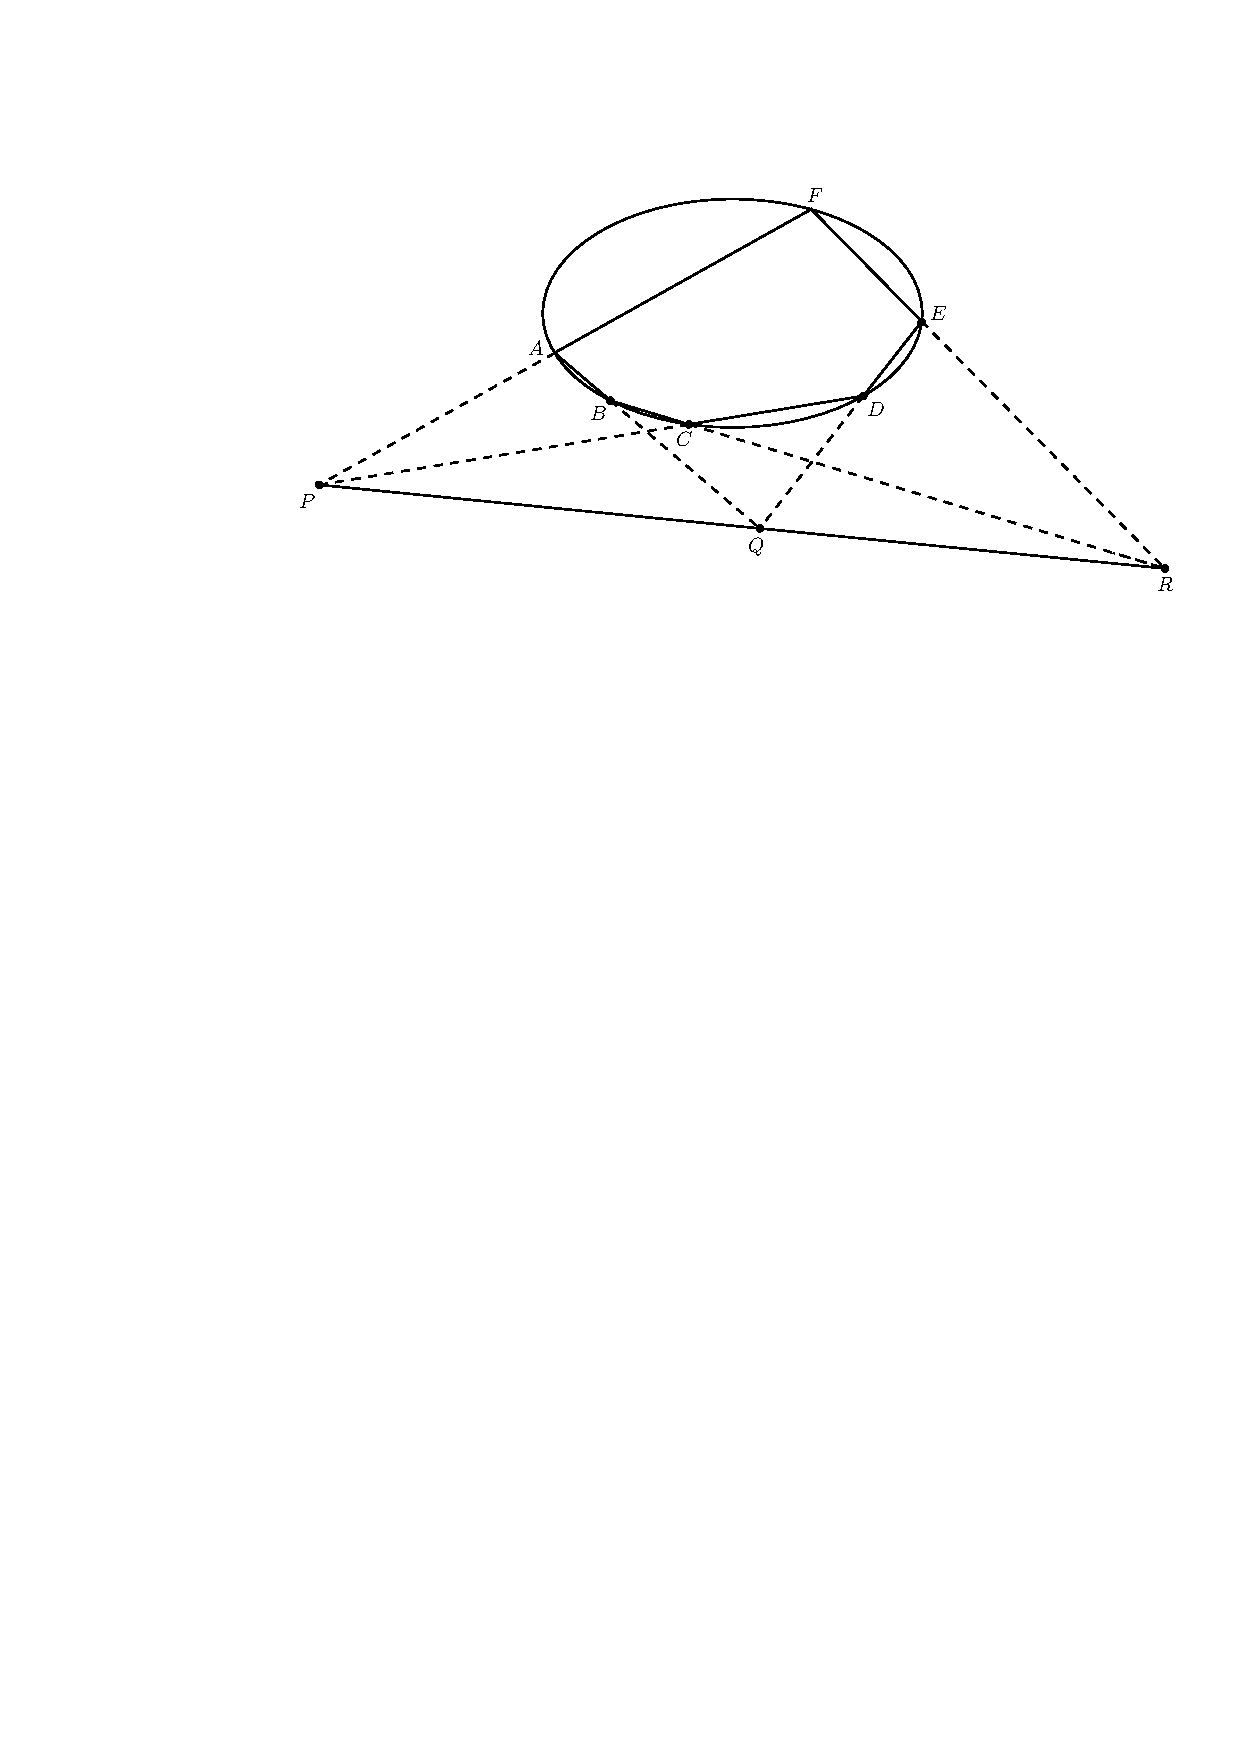
\includegraphics[width=250pt]{pictures/pascal-thm}
\caption{The mystic hexagon.}
\end{figure}
\begin{proof}
In the diagram, consider the two triples of lines
\[L_1:PAF,\quad L_2:QDE,\quad L_3:RBC.\]
and 
\[M_1:PCD,\quad M_2:QAB,\quad M_3:REF.\]
let $C_1=L_1+L_2+L_3$ and $C_2=M_1+M_2+M_3$. Now clearly $C_1$ and $C_2$ are two cubics such that
\[C_1\cap C_2=\{A,B,C,D,E,F,P,Q,R\}.\]
Suppose $PQR$ are collinear, with $L=PQR$, let $\Gamma$ be the conic through $ABCDE$ (the existence and unicity of which is provided by Proposition~\ref{conic dim}). Then by construction, $L+\Gamma$ is a cubic passing through the $8$ points $A,B,C,D,E,P,Q,R$, and by Corollary~\ref{cubic 9 point}, it must contain $F$. By assumption, $F\notin L$, since otherwise $A,E,F$ would by collinear, so necessarily we have $F\in\Gamma$, proving that the six points are conconic.\par
Now conversely, suppose that $ABCDEF$ are on a nondegenerate conic $\Gamma$, and let $L=PQ$; then is a cubic passing through $A,B,C,D,E,F,P,Q$, so by Corollary~\ref{cubic 9 point} it must pass through $R$. Now $R$ can't be on the conic $\Gamma$ (since otherwise the points $F,E,R$ is colliearly in $\Gamma$, and thus $\Gamma$ is a line pair, contradiction), so $R\in L$, that is, $PQR$ are collinear.
\end{proof}
\section{Tangent space and nonsingularity}
\subsection{Nonsingular points of a hypersurface}
Suppose $f\in k[X_1,\dots,X_n]$ is irreducible, $f\notin k$, and set $V=V(f)\sub\mathbb{A}^n$; let $P=(a_1,\dots,a_n)\in V$, and $\ell$ be a line through $P$. Since $P\in V$, obviously $P$ is a root of $f|_{\ell}$. When is $P$ a multiple root of $f|_{\ell}$?
\begin{proposition}
The point $P$ is a multiple root of $f|_{\ell}$ if and only if the line $\ell$ is contained in the affine linear subspace $T_PV$ defined by the equation
\[\sum_i\frac{\partial f}{\partial X_i}(P)(X_i-a_i)=0,\]
called the \textbf{tangent space} to $V$ at $P$. We say that every line
contained in $T_PV$ and passing through $P$ is \textbf{tangent to $\bm{V}$ at $\bm{P}$}. If $\partial f/\partial X_i(P)=0$ for all $i$, we say that each line passing
through $P$ is tangent to $V$ at $P$.
\end{proposition}
\begin{proof}
We consider parametric equations for $\ell$ of the form $X_i=a_i+b_it$, where $(b_1,\dots,b_n)$ is the direction vector of $\ell$. Then $f|_{\ell}=f(\dots,a_i+b_it,\dots)=:g(t)$ is a polynomial in $t$, and we know that $t=0$ is one root of $g$. Hence
\[\text{$0$ is a multiple root of $g$}\iff\frac{\partial g}{\partial t}(0)=0,\]
that is,
\[\sum_ib_i\frac{\partial f}{\partial X_i}(P)=0.\]
This condition is equivalent to the fact that $\ell\sub T_PV$.
\end{proof}
\begin{definition}
A point $P\in V\sub\mathbb{A}^n$ is a \textbf{nonsingular point} of $V$ if $\partial f/\partial X_i(P)\neq 0$ for some $i$; otherwise $P$ is a \textbf{singular point}, or a \textbf{singularity} of $V$.
\end{definition}
Obviously $T_PV$ is an $(n-1)$-dimensional affine subspace of $\mathbb{A}^n$ if $P$ is nonsingular, and $T_PV=\mathbb{A}^n$ if $P\in V$ is singular.
\begin{remark}
Suppose that $k=\R$ or $\C$, and suppose for example that $\partial f/\partial x_1(P)\neq0$. Consider the map $p:\mathbb{A}^n\to\mathbb{A}^n$ defined by $(X_1,\dots,X_n)\mapsto(f,X_2,\dots,X_n)$. The determinant of the Jacobian matrix
\[\begin{pmatrix}
\dfrac{\partial f}{\partial X_1}&\dfrac{\partial f}{\partial X_2}&\cdots&\dfrac{\partial f}{\partial X_n}\\[8pt]
0&1&\cdots&0\\[4pt]
0&0&\cdots&1
\end{pmatrix}\]
is non-zero at $P$. Thus, by the inverse function theorem, there exists a neighborhood $U\sub\mathbb{A}^n$, $P\in U$, such that the restriction $p|_U:U\to p(U)\sub\mathbb{A}^n$ is a diffeomorphism from $U$ to open set $p(U)$ in the usual Euclidean topology of $\R^n$ or $\C^n$.\par
In other words, $(f,X_2,\dots,X_n)$ is a new system of coordinates on $\mathbb{A}^n$ near to $P$. This implies that an euclidean neighborhood of $P$ in the hypersurface $V$ of equation $f=0$ is diffeomorphic to an open set in $\mathbb{A}^{n-1}$ with coordinates $(Y_2,\dots,Y_n)$. We express this fact by saying that close to the non-singular point $P$ the non-singular variety $V$ has $(Y_2,\dots,Y_n)$ as \textbf{local parameters}.
\end{remark}
Let us consider the set
\[V_{nonsin}=\{P\in V:\text{$P$ is nonsingular}\}\]
of non-singular points of $V$.
\begin{proposition}\label{hypersurface nonsin dense}
$V_{nonsin}$ is a dense open set of $V$ for the Zariski topology.
\end{proposition}
\begin{proof}
The set $V_{sin}$ of singular points is defined by $\partial f/\partial X_i=0$ for all $i$, that is,
\[V_{\sin}=V\Big(f,\frac{\partial f}{\partial X_1},\dots,\frac{\partial f}{\partial X_n}\Big).\]
which is closed by definition of the Zariski topology. Since $V$ is irreducible, to show that the open $V_{nonsin}$ is dense, we only have to show it's nonempty; arguing by contradiction, suppose that it's empty, that is, suppose $V=V(f)=V_{sin}$. Then each of the polynomials $\partial/\partial X_i$ must vanish on $V$, therefore they must be divisible by $f$ in $k[X_1,\dots,X_n]$; but viewed as a polynomial in $X_i$, $\partial f/\partial X_i$ has degree strictly smaller than $f$, so that $f$ divides $\partial f/\partial X_i$ implies that in fact $\partial f/\partial X_i=0$ as a polynomial. Over $\C$, this is obviously only possible if $X_i$ does not appear in $f$, and if this happens for all $i$ then $f$ is constant, which is excluded. Over a general field $k$, $\partial f/\partial X_i=0$ is only possible if $f$ is an inseparable polynomial in $X_i$, that is, $\char k=p$, and $X_i$ only appears in $f$ as the $p$-th power $X^p_i$. If this happens for each $i$, then by the argument given in Proposition~\ref{Noe normal adjust}, $f$ is a $p$-th power in $k[X_1,\dots,X_n]$, this contradicts the fact that $f$ is irreducible.
\end{proof}
We can now define the tangent space to an affine algebraic set $V$ at one of its points, and study some properties related to the concept of dimension.
\begin{definition}
Let $V\sub\mathbb{A}^n$ be a variety, with $P=(a_1,\dots,a_n)\in V$. For any $f\in k[X_1,\dots,X_n]$, write
\[f^{(1)}_P=\sum_i\frac{\partial f}{\partial X_i}(P)(X_i-a_i).\]
This is an affine linear polynomial, the first order part of $f$ at $P$. Now define the \textbf{tangent space to $\bm{V}$ at $\bm{P}$} by
\[T_PV=\bigcap_{f\in I(V)}(f_P^{(1)}=0).\]
\end{definition}
If $V=V(J)$ (where we can always suppose that $J$ is a radical ideal and so $J=I(V)$) one sees immediately that the linear parts of the polynomials of $J$ generate an ideal $J_P^{(1)}=\{f_P^{(1)}:f\in J\}$ and so
\[T_PV=V(J^{(1)}_P).\]
Let $I(V)=(f_1,\dots,f_m)$. Since the linear part of the sum of two polynomials is the sum of the linear parts of the two summands, one has that for each $g\in I(V)$, the linear part $g^{(1)}_P$ of $g$ in $P$ is a linear combination of those of the $f_i$. Therefore, $J^{(1)}_P=(f_{1,P}^{(1)},\dots,f^{(1)}_{m,P})$. Hence the definition of $T_PV$ becomes simply
\[T_PV=V(f_{1,P}^{(1)},\dots,f^{(1)}_{m,P})=\bigcap_{i=1}^{m}V(f^{(1)}_{i,P})\]
\begin{proposition}
The function $V\to\N$ defined by $P\mapsto\dim T_PV$ is an upper semi-continuous function in the Zariski topology of $V$. In other words, for any integer $r$, the subset
\[S(r)=\{P\in V\mid\dim T_PV\geq r\}\]
is closed.
\end{proposition}
\begin{proof}
Let $(f_1,\dots,f_m)$ be a set of generators of $I(V)$. Then
\[T_PV=V(f_{1,P}^{(1)},\dots,f^{(1)}_{m,P})=\bigcap_{i=1}^{m}V(f^{(1)}_{i,P}).\]
That is, $T_PV$ is the zero set of the function $f:\mathbb{A}^n\to\mathbb{A}^m$ defined by
\[(X_1,\dots,X_n)\mapsto(f^{(1)}_{1,P},\dots,f^{(1)}_{m,P}).\]
Since $f^{(1)}_{i,P}$ are linear forms, the map $f$ has constant rank, so that we get $\dim T_PV=n-\rank\partial f$. This implies
\[P\in S(r)\iff\rank\Big(\frac{\partial f_i}{\partial X_j}(P)\Big)\leq n-r.\]
Now each entry $\partial f_i/\partial X_j$ of the matrix is a polynomial function of $P$, thus each minor is a determinant of a matrix of polynomials, and so is itself a polynomial. Hence $S(r)\sub V\sub\mathbb{A}^n$ is an algebraic subset.
\end{proof}
\begin{corollary}
There exists an integer $r$ and a dense open subset $V_0\sub V$ such that
\[\dim T_PV=r\text{ for }P\in V_0\And \dim T_PV\geq r\text{ for all $P\in V$}.\]
Define $r$ to be the \textbf{dimension of $\bm{V}$}, and write $\dim V=r$. We say that $P\in V$ is \textbf{nonsingular} if $\dim T_PV=r$, and \textbf{singular} if $\dim T_PV>r$. A variety $V$ is nonsingular if it is nonsingular at each point. The closed subset $V_{sin}$, the locus of the singular points of $V$, is the \textbf{singular locus} of $V$; it is empty if $V$ is non-singular.
\end{corollary}
\begin{proof}
Let $r=\min_{P\in V}\{\dim T_PV\}$. Then clearly
\[S(r-1)=\emp,\quad S(r)=V,\quad S(r+1)\subset V.\]
Therefore $S(r)-S(r+1)=\{P\in V\mid \dim T_PV=r\}$ is open and nonempty.
\end{proof}
\subsection{Dimension equals transcendence degree-the hypersurface case}
\begin{definition}
If $k\sub K$ is an extension of fields, the \textbf{transcendence degree} of $K$ over $k$ is the maximal number of elements of $K$ that are algebraically independent over $k$. It is indicated by $\tr\deg_kK$.
\end{definition}
It follows from Proposition~\ref{hypersurface nonsin dense} that if $V=V(f)\sub\mathbb{A}^n$ is a hypersurface defined by some nonconstant irreducible polynomial $f$, then $\dim V=n-1$. We now prove that $\tr\deg_kk(V)=n-1$; from this it follows, in particular, that for a hypersurface $V$,
\[\dim V=\tr\deg_kk(V)=n-1.\]
Consider the quotient mapping
\[\pi:k[X_1,\dots,X_n]\to k[V]=k[X_1,\dots,X_n]/(f)\]
and let $x_i=\pi(X_i)$. Suppose, to fix our ideas, that the indeterminate
$X_1$ actually appears in $f$ and consider the elements $x_2,\dots,x_n\in k(V)$. If one had $\tr\deg_kk(V)<n-1$, they would be algebraically dependent and so there would exist a polynomial $g(X_2,\dots,X_n)\in k[X_2,\dots,X_n]$ such that
\[g(X_2,\dots,X_n)=0.\]
that is, $g\in(f)$. But that is absurd because $X_1$ does not appear in $g$. Hence $\tr\deg_kk(V)\geq n-1$. Since one certainly has $\tr\deg_kk(V)<n$, it follows that $\tr\deg_kk(V)=n-1$.\par
The rest of this section is concerned with proving that the equality $\dim V=\tr\deg_kk(V)$ holds for all varieties, by reducing to the case of a hypersurface. The first thing to show is that for a point $P\in V$ of a variety, the tangent space $T_PV$, which so far has been discussed in terms of a particular coordinate system in the ambient space $\mathbb{A}^n$, is in fact an intrinsic property of a neighbourhood of $P\in V$.
\subsection{Intrinsic nature of \boldmath$T_PV$}
From now on, given $P=(a_1,\dots,a_n)\in V\sub\mathbb{A}^n$, we take new coordinate $X'_i=X_i-a_i$ to bring $P$ to the origin, and thus assume that $P=(0,\dots,0)$. Then $T_PV\sub\mathbb{A}^n$ is a vector subspace of $k^n$. Let $\m_P$ be the maximal ideal of $P$ in $k[V]$, and 
\[M_P=(X_1,\dots,X_n)\sub k[X_1,\dots,X_n].\]
Then of course $\m_P=M_P/I(V)\sub k[V]$.
\begin{theorem}
With the above notation,
\begin{itemize}
\item[$(1)$] There is a natural isomorphism of vector spaces
\[(T_PV)^*=\m_P/\m_P^2.\]
where $(T_PV)^*$ denotes the dual space.
\item[$(2)$] If $f\in k[V]$ is such that $f(P)\neq0$, and $V_f\sub V$ is the standard affine open, then the natural map
\[T_P(V_f)\to T_PV\]
is an isomorphism.
\end{itemize}
\end{theorem}
\begin{proof}
Write $(k^n)^*$ for the vector space of linear forms on $k^n$, this is the vector space with basis $X_1,\dots,X_n$. Since $P=(0,\dots,0)$, for any $f\in k[X_1,\dots,X_n]$, the linear part $f^{(1)}_P$ is naturally an element of $(k^n)^*$. Consider the map
\[d:M_P\to (k^n)^*\]
defined by putting $df=f^{(1)}_P$ for each $f\in M_P$.\par
The map $d$ is obviously surjective. Indeed, the linear forms $X_1,\dots,X_n\in (k^n)^*$ are the images of the elements $X_1,\dots,X_n\in M_P$. Moreover $\ker d=M_P^2$ since $f^{(1)}_P=0$ if and only if $f$ has quadratic terms in $X_1,\dots,X_n$ in minimal degree; that is, if and only if $f\in M_P^2$. Thus
\[(k^n)^*=M_P/M_P^2.\]
This proves $(1)$ in the particular case $V=\mathbb{A}^n$.\par
In the general case one has the restriction map $(k^n)^*\to(T_PV)^*$, dual to the inclusion $T_PV\sub k^n$, which sends a linear form $\lambda$ on $k^n$ into its restriction to $T_PV$. By composition one obtains a map
\[D:M_P\to (k^n)^*\to(T_PV)^*.\]
The composite $D$ is surjective since each factor is. It suffices to prove that
\[\ker D=M_P^2+I(V).\]
because from this it follows that
\[\m_P/\m_P^2=M_P/(M_P^2+I(V))\cong (T_PV)^*.\]
To prove the claim, note that
\[f\in\ker D\iff f^{(1)}_P|_{T_PV}=0\iff f_P^{(1)}=\sum_ia_ig_{i,P}^{(1)}\text{ for some $g_i\in I(V),a_i\in k[X_1,\dots,X_n]$}.\]
The last condition is equivalent to 
\[f-\sum_ia_ig_i\in M_P^2\text{ for some $g_i\in I(V),a_i\in k[X_1,\dots,X_n]$}.\]
which means that $f\in M_P^2+I(V)$.\par
To prove $(2)$ we use the identification $V_f\cong V(I(V),Yf-1)\sub\mathbb{A}^{n+1}$. Then $I(V_f)=(I(V),Yf-1)\sub k[X_1,\dots,X_n,Y]$, and the point $P=(0,\dots,0)$ is mapped to $(0,\dots,0,1/f(P))$. With the observation
\[(Yf-1)^{(1)}_{P}=Yf^{(1)}_P+f(Y-1/f(P)),\]
we can see that $T_P(V_f)\sub\mathbb{A}^{n+1}$ is defined by the equations defining $T_PV$ plus the equation 
\[Yf^{(1)}_P+f(Y-1/f(P))=0.\]
Thus the natural map 
\[T_P(V)\mapsto T_P(V_f),\quad P\mapsto(P,1/f(P))\]
is an inverse of the morphism $T_P(V_f)\to T_PV$.
\end{proof}
\begin{corollary}
$T_PV$ only depends on a neighbourhood of $P\in V$ up to isomorphism. More precisely, if $P\in V_0\sub V$ and $Q\in W_0\sub W$ are open subsets of affine varieties, and $\varphi:V_0\to W_0$ is an isomorphism taking $P$ into $Q$, there is a natural isomorphism $T_PV\to T_PW$; hence $\dim T_PV=\dim T_QW$.\par
In particular, if $V$ and $W$ are birationally equivalent varieties then $\dim V=\dim W$.
\end{corollary}
\begin{proof}
By passing to a smaller neighbourhood of $P$ in $V$, we can assume $V_0$ is isomorphic to an affine variety. Then so is $W_0$, and $\varphi$ induces an isomorphism $k[V_0]\cong k[W_0]$ taking $\m_P$ into $\m_Q$. Therefore, $\m_P/\m_P^2\cong\m_Q/\m_Q^2$ and $T_PV\cong T_QW$.\par
The final sentence holds because by Proposition~\ref{biration equiv iff}, $V$ and $W$ contain dense open subsets which are isomorphic.
\end{proof}
\begin{theorem}
For any affine variety $V$,
\[\dim V=\tr\deg_kk[V].\]
\end{theorem}
\begin{proof}
This is known if $V$ is a hypersurface. On the other hand, every variety is birational to a hypersurface by Proposition~\ref{hypersurface reduction}, and both sides of the required relation are the same for birationally equivalent varieties.
\end{proof}
\subsection{Dimension of varieties}
In view of the dimension of affine varieties, we make the following definition.
\begin{definition}
The dimension of an projective variety $V$ is the transcendence degree of the function field $k(V)$; it is denoted by $\dim V$. The dimension of a reducible algebraic set is the maximum of the dimension of its irreducible components. If $W\sub V$ is a closed subvariety of $V$ then the number $\dim V-\dim W$ is called the codimension of $W$ in $V$, and written $\codim W$ or $\codim_VW$. Algebraic varieties of dimension $1$ and $2$ are called \textbf{curves} and \textbf{surfaces}.
\end{definition}
Note that if $X$ is an irreducible variety and $U\sub X$ is open then $k(U)=k(X)$, and hence $\dim U=\dim X$.
\begin{example}
$\dim\mathbb{A}^n=\dim\P^n=n$, because the field $k(\mathbb{A}^n)$ is the field of rational functions in $n$ variables. Since dimension is by definition invariant under birational equivalence, we see that $\mathbb{A}^n$ and $\mathbb{A}^m$ are not birational if $n\neq m$.
\end{example}
\begin{example}
If $V$ consists of a single point then obviously $\dim V=0$, and thus the same holds if $V$ is a finite set. Conversely, if $\dim V=0$ then $V$ is a finite set. It is enough to prove this for an affine variety $V$. Let $V\sub\mathbb{A}^n$ and write $x_1,\dots,x_n$ for the coordinates on $\mathbb{A}^n$ as functions on $V$, that is, as elements of $k[V]$. By assumption the $x_i$ are algebraic over $k$, and can hence only take finitely many values. It follows from this that $V$ is finite.
\end{example}
\begin{proposition}
If $X$ and $Y$ are varieties then
\[\dim(X\times Y)=\dim X+\dim Y.\]
\end{proposition}
\begin{proof}
We need only consider the case that $X\sub\mathbb{A}^N$ and $Y\sub\mathbb{A}^M$ are affine varieties. Suppose that $\dim X=n,\dim Y=m$, and let $x_1,\dots,x_N$ and $y_1,\dots,y_M$ be coordinates of $\mathbb{A}^N$ and $\mathbb{A}^M$ considered as functions on $X$ and $Y$ respectively, such that $t_1,\dots,t_n$ are algebraically independent in $k(X)$ and $y_1,\dots,y_m$ in $k(Y)$. By definition $k[X\times Y]$ is generated by the elements $x_1,\dots,x_N,y_1,\dots,y_M$, and under the current assumptions all of these are algebraically dependent on $x_1,\dots,x_n,y_1,\dots,y_m$. Hence it is enough to prove that these elements are algebraically independent. Suppose that there is a relation $F(X,Y)=F(X_1,\dots,X_n,Y_1,\dots,Y_m)=0$ on $X\times Y$. Then for any point $x\in X$ we have $F(x,Y_1,\dots,Y_m)=0$ on $Y$. Since $y_1,\dots,y_m$ are algebraically independent in $k(Y)$, every coefficient $a_i(x)$ of the polynomial $F(x,Y)$ is zero; this means that the corresponding polynomial $a_i(X_1,\dots,X_n)$ is $0$ on $X$. Now we use the fact that $x_1,\dots,x_n$ are algebraically independent in $k(X)$ and deduce from this that $a_i(Y_1,\dots,Y_n)=0$, and hence $F(X,Y)$ is identically 0.
\end{proof}
\begin{theorem}\label{dimension monotone}
Let $Y$ be a variety. If $X$ is a closed subset of $Y$ with $\dim X=\dim Y$ then $X=Y$.
\end{theorem}
\begin{proof}
It is enough to prove the assertions for affine varieties.\par
Suppose $X\sub Y\sub\mathbb{A}^N$ with $\dim Y=n$. Then any $n+1$ of the coordinate functions $t_1,\dots,t_N$ are algebraically dependent as elements of $k[Y]$, that is, are connected by a relation $F(t_{i_1},\dots,t_{i_{n+1}})=0$ on $Y$. A fortiori this holds on $X$. This means that the transcendence degree of $k(X)$ is at most $n$, so that $\dim X\leq\dim Y$.\par
Now suppose that $\dim X=\dim Y=n$. Then some $n$ of the coordinates $x_1,\dots,x_n$ are algebraically independent on $X$; suppose that these are $x_1,\dots,x_n$. Then a fortiori they are algebraically independent on $Y$. Let $f\in k[Y]$ with $f\neq 0$ on $Y$. Then $f$ on $Y$ is algebraically dependent on $x_1,\dots,x_n$, that is, there is a relation on $Y$ of the form
\[h_0(x_1,\dots,x_n)f^k+\cdots+h_k(x_1,\dots,x_n)=0\]
where we can choose such that $h_k(x_1,\dots,x_n)\neq 0$ on $Y$. This equation holds a fortiori on $X$. Suppose that $f=0$ on $X$, so that $h_k(x_1,\dots,x_n)=0$ on $X$. Since by assumption $x_1,\dots,x_n$ are independent on $X$, it follows that $h_k(x_1,\dots,x_n)=0$ on the whole of $\mathbb{A}^N$. This is a contradiction. Thus if $f=0$ on $X$ then also $f=0$ on $Y$, and therefore $X=Y$. The theorem is proved.
\end{proof}
We have seen that an irreducible algebraic plane curve is $1$-dimensional. The
following result is a generalisation.
\begin{theorem}
Every irreducible component of a hypersurface in $\mathbb{A}^n$ or $\P^n$ has codimension $1$.
\end{theorem}
\begin{proof}
It is enough to consider the case of a hypersurface in $\mathbb{A}^n$. Suppose that a variety $X\sub\mathbb{A}^n$ is given by an equation $F(X)=0$. The factorisation $F=F_1\cdots F_r$ of $F$ into irreducible factors corresponds to an expression $V=V_1\cup\cdots\cup V_k$, where $V_i=V(F_i)$. By Corollary~\ref{hypersurface decomposition} this is the decomposition of $V$. Suppose that the variable $X_n$ actually appears in the polynomial $F_i(X)$, we prove that the coordinates $x_1,\dots,x_{n-1}$ are algebraically independent on $V_i$. Indeed, a relation $G(t_1,\dots,t_{n-1})=0$ on $V_i$ would imply that $G^\ell\in(F_i)$ for some $\ell>0$, which is impossible since $G$ does not involve $X_n$. Thus $\dim V_i\geq n-1$; since $V\neq\mathbb{A}^n$, it follows from Theorem~\ref{dimension monotone} that $\dim V_i=n-1$.
\end{proof}
Here is a converse of the previous theorem.
\begin{theorem}
Let $V\sub\mathbb{A}^n$ be an algebraic subset, and suppose that all the components of $V$ have dimension $n-1$. Then $V$ is a hypersurface and the ideal $I(V)$ is principal.
\end{theorem}
\begin{proof}
We only need consider the case that $V$ is irreducible. Since $V\neq\mathbb{A}^n$ (because $\dim V=n-1$), there exists a nonzero polynomial $F$ which is zero on $V$. Since $V$ is irreducible, some irreducible factor $H$ of $F$ is also zero on $V$. Write $W\sub\mathbb{A}^n$ for the hypersurface defined by $H=0$; we saw that $W$ is irreducible. Then $V\sub W$, so that $V=W$ by Theorem~\ref{dimension monotone}. Now by nullstellensatz $I(V)=I(V(H))=(H)$.
\end{proof}
The following analogue is proved similarly:
\begin{theorem}
Let $X\sub\P^{n_1}\times\cdots\times\P^{n_k}$ be an algebraic subset, and suppose that all the components of $X$ have dimension $n_1+\cdots+n_k-1$. Then $X$ is defined by one equation that is homogeneous in each of the $k$ sets of variables.
\end{theorem}